\documentclass[fontsize=12pt]{scrartcl}

%Settings-Datei einbinden
% !TEX root = Bachelorarbeit_Paul_Zilewitsch.tex
\usepackage{comment}
\usepackage{amsmath}
\usepackage{amssymb}

% deutsche Silbentrennung
\usepackage[ngerman]{babel}

% deutsche Umlauten
\usepackage[T1]{fontenc}
\usepackage{inconsolata}
\usepackage[utf8]{inputenc}

%Anführungszeichen
\usepackage[autostyle=true,german=quotes]{csquotes}

%Zeilenabstand 1,5 
\usepackage[onehalfspacing]{setspace}

%Times New Roman
\usepackage{mathptmx}
\setkomafont{disposition}{\rmfamily}

%Arrays, Tabellen und Listen
\usepackage{array}
\usepackage{tabto}
\usepackage{longtable}
\usepackage{supertabular}

%Seitenzahlen
\usepackage{scrpage2}
\cfoot[]{}
\ofoot[\pagemark]{\pagemark}
\pagestyle{scrheadings}

%Inhaltsverzeichnis
\usepackage{tocloft}
\usepackage{titletoc}
\cftsetindents{section}{0.0in}{0.5in}
\cftsetindents{subsection}{0.0in}{0.5in}
\cftsetindents{subsubsection}{0.0in}{0.5in}
\cftsetindents{paragraph}{0.0in}{0.5in}
\renewcommand{\cftsecleader}{\cftdotfill{\cftdotsep}}
\renewcommand\cftsecfont{\mdseries}
\renewcommand\cftsecpagefont{\mdseries}
\renewcaptionname{ngerman}{\contentsname}{} %kein Titel für Inhaltsv. 
%\usepackage{hyperref} %für links im inhaltsverzeichnis

%Abkürzungsverzeichnis
\usepackage{enumitem} 

%Abbildungsverzeichnis
\renewcaptionname{ngerman}{\listfigurename}{}

\titlecontents{figure}
  [0em]
  {}
  {\figurename\enspace\thecontentslabel:\enspace}
  {}
  {\titlerule*[1pc]{.}\contentspage}
  
  %Tabellenverzeichnis
\renewcaptionname{ngerman}{\listtablename}{}

\titlecontents{table}
  [0em]
  {}
  {\tablename\enspace\thecontentslabel:\enspace}
  {}
  {\titlerule*[1pc]{.}\contentspage}

%Seitenränder
\usepackage{geometry}
\geometry{a4paper, top=21mm, left=30mm, right=20mm, bottom=20mm,
headsep=10mm, footskip=10mm}

%C# Code-Anzeige
\usepackage{color}
\definecolor{bluekeywords}{rgb}{0.13,0.13,1}
\definecolor{greencomments}{rgb}{0,0.5,0}
\definecolor{redstrings}{rgb}{0.9,0,0}

\usepackage{listings}
\lstset{language=[Sharp]C,
  showspaces=false,
  showtabs=false,
  breaklines=true,
  showstringspaces=false,
  breakatwhitespace=true,
  escapeinside={(*@}{@*)},
  commentstyle=\color{greencomments},
  keywordstyle=\color{bluekeywords},
  stringstyle=\color{redstrings},
  basicstyle=\ttfamily
}

%Überschriften Definition
\usepackage{titlesec}

\titleformat{\section}
  {\normalfont\fontsize{16}{17}\rmfamily\bfseries}
  {\thesection}
  {2em}
  {}

\titleformat{\subsection}
  {\normalfont\fontsize{14}{17}\rmfamily\bfseries}
  {\thesubsection}
  {1.5em}
  {}
  
  \titleformat{\subsubsection}
  {\normalfont\fontsize{14}{17}\rmfamily\mdseries}
  {\thesubsubsection}
  {0.75em}
  {}
\titlespacing{\section}{0pt}{*6}{*5} %{Einzug} {abstand nach oben}{abstand nach unten}
\titlespacing{\subsection}{0pt}{*5}{*3}
\titlespacing{\susubbsection}{0pt}{*4}{*2}

%Fußnoten
\usepackage[multiple, hang]{footmisc} % Komma zwischen mehreren Fußnoten
\setlength{\footnotemargin}{1em}
%\usepackage[justification=RaggedRight, singlelinecheck=false]{caption}
%\usepackage{caption}
%\captionsetup{%
%  textfont=footnotesize,
%  labelfont=footnotesize,
%  font=singlespacing,
%}


%Bilder
\usepackage{graphicx}


%Farben und Zeichnungen
\usepackage{pict2e}  
\usepackage{color}
\usepackage{ amssymb }
\definecolor{gray}{RGB}{150, 150, 150}


%Literaturverzeichnis
%\bibliographystyle{apalike} 
\bibliographystyle{unsrtnat} 
\usepackage[numbers,round,sort]{natbib}
\addto\captionsngerman{\renewcommand{\refname}{Literaturverzeichnis}}






\begin{document}

%-------------------------------------------------------------------------------------------------------
%					Titelseite
%-------------------------------------------------------------------------------------------------------
\thispagestyle{empty}
\large
	\noindent Berufsakademie Sachsen \hfill KMS Computer GmbH\\
	Staatliche Studienakademie Dresden\\
	Studiengang Informationstechnik 
\begin{center}	
	\vspace*{4cm}
	\textbf{Konzipierung und prototypische Entwicklung einer E-Mail Integration auf Basis der Microsoft Exchange Web Services im Service Desk der CAFM Software GEBman 10}\\
	\vspace*{2cm}
		Bachelorarbeit\\ zur Erlangung des Abschlusses\\ Bachelor of Engineering\\ im Studiengang 						Informationstechnik \\
	\vspace*{2cm}
	eingereicht von:\\Zilewitsch, Paul
	\vspace*{3cm}
\end{center}
	1. Gutachter: Dr. rer. nat. Dipl.-Chem. Hansi Schilling\\
	2. Gutachter: B.Sc. Sebastian Schulze 
	\\\\
	\begin{tabular}{@{}ll}
		Tag der Themenübergabe:&22.04.2016\\
		Tag der Einreichung:&18.07.2016
	\end{tabular}
\pagebreak


%-------------------------------------------------------------------------------------------------------
%					Auftragsblatt wird mit abgeheftet und mitgezählt
%-------------------------------------------------------------------------------------------------------



%-------------------------------------------------------------------------------------------------------
%					Autorenreferat
%-------------------------------------------------------------------------------------------------------
\noindent
\Large\bfseries
Autorenreferat
\normalsize\mdseries
\thispagestyle{empty}
\newline\newline
\noindent
ZILEWITSCH, Paul: Konzipierung und prototypische Entwicklung einer E-mail Integration auf Basis der Microsoft Exchange Web Services im Service Desk der CAFM Software GEBman 10,  Berufsakademie Sachsen, Staatliche Studienakademie Dresden, Studiengang Informationstechnik, Bachelorarbeit, 2016.\\ 
41 Seiten, 42 Literaturquellen , 4 Anlagen. \\\\\\\\

\noindent
Die KMS Computer GmbH entwickelt seit 2011 die Webanwendung GEBman 10. Diese Webanwendung besitzt über 40 Module. Eines davon ist das Modul Service Desk. Ziel der vorliegenden Arbeit ist es, Verbesserungsmöglichkeiten dieses Service Desk-Moduls festzuhalten. Dadurch könnte es als Service Desk-Softwarelösung des Supports der KMS Computer GmbH dienen und auf eine externe Lösung verzichtet werden. Hierfür werden verschiedene, auf dem Markt befindliche, Service Desk-Softwarelösungen analysiert und ausgewertet, um anschließend Verbesserungsmöglichkeiten für das Service Desk-Modul identifizieren zu können.\newline
Außerdem soll die E-Mail Integration des Service Desk-Moduls erweitert werden. Dabei wird auf die bereits vorhandenen Funktionalitäten in GEBman 10 zurückgegriffen, die auf den Microsoft Exchange Web Services basieren.

\newpage

%-------------------------------------------------------------------------------------------------------
%					Inhaltsverzeichnis
%-------------------------------------------------------------------------------------------------------
\addsec{Inhaltsverzeichnis} %vergebe keine Kapitelnummer\\
\vspace*{-1cm}
\pagenumbering{Roman}
\setcounter{page}{4}
\tableofcontents
\newpage

%-------------------------------------------------------------------------------------------------------
%					Abbildungsverzeichnis
%-------------------------------------------------------------------------------------------------------
\addsec{Abbildungsverzeichnis} %vergebe keine Kapitelnummer
\vspace*{-1cm}
\begin{spacing}{1.8}
\listoffigures
\end{spacing}
\newpage

%-------------------------------------------------------------------------------------------------------
%					Abkürzungsverzeichnis
%------------------------------------------------------------------------------------------------------
\addsec{Abkürzungsverzeichnis} %vergebe keine Kapitelnummer

\noindent
API \tabto{4cm} Application Programming Interface\\

\noindent
CAFM \tabto{4cm} Computer-Aided Facility Management\\

\noindent
HTTP \tabto{4cm} Hypertext Transfer Protocol\\

\noindent
HTTPS \tabto{4cm} Hypertext Transfer Protocol Secure\\

\noindent
ITIL \tabto{4cm} Information Technology Infrastructure Library\\

\noindent
REST API \tabto{4cm} Representational State Transfer Application Programming Interface\\

\noindent
SOAP \tabto{4cm} Simple Object Access Protocol\\

\noindent
SPoC \tabto{4cm} Single Point of Contact\\

\noindent
UML \tabto{4cm} Unifed Modeling Language\\

\noindent
XML \tabto{4cm} Extensible Markup Language\\

\noindent
XSS \tabto{4cm} Cross-Site-Scripting
\newpage

%-------------------------------------------------------------------------------------------------------
%					Tabellenverzeichnis
%-------------------------------------------------------------------------------------------------------
\addsec{Tabellenverzeichnis} %vergebe keine Kapitelnummer
\vspace*{-1cm}
\begin{spacing}{1.8}
\listoftables
\end{spacing}
\newpage

%-------------------------------------------------------------------------------------------------------
%					1	Einleitung
%-------------------------------------------------------------------------------------------------------


\pagenumbering{arabic}     
\setcounter{page}{1}
% !TEX root = Bachelorarbeit_Paul_Zilewitsch.tex
\section{Einleitung}

%http://webuser.hs-furtwangen.de/~kaspar/seminar0405/Service_Desk.pdf

\subsection{Die Software GEBman 10 von der KMS Computer GmbH}
\noindent
Die IT ist ein ständiger Begleiter im Arbeitsalltag eines jeden Unternehmens. Sie erleichtert nicht nur die Arbeit mit großen Datenmengen, sondern unterstützt auch wichtige Geschäftsprozesse in -und außerhalb des Unternehmens. Um einen möglichst effizienten Einsatz der IT zu ermöglichen, halten sich viele Unternehmen an bestimmte Best Practice Frameworks. Diese Leitfäden beinhalten unter anderem den Einsatz der IT im Bereich Kundenservice. Dabei übernimmt ein sogenannter Service Desk eine wichtige Funktion. Diese zentrale Anlaufstelle dient als Kommunikationsschnittstelle zwischen dem Kunden und der IT-Organisation. Viele Unternehmen setzen auf eine externe Service Desk-Softwarelösung, die dem Support eine bessere Kommunikation mit dem Kunden und ein effizienteres Abarbeiten von Vorfällen ermöglicht.\\

\noindent
Die KMS Computer GmbH bietet ebenfalls eine Lösung eines Service Desk an, die jedoch auf den Bereich Facility Management spezialisiert ist. Das Unternehmen wurde 1990 gegründet und konzentriert sich heute vorrangig auf den Vertrieb von entwickelter Software im Bereich Computer-Aided Facility Management (CAFM). Computer-Aided bedeutet so viel wie \enquote{computergestützt}. Den Begriff Facility Management beschreibt der Spezialist für Gebäude- und Immobilienwirtschaft Nävy präzise \enquote{als strategische Management-Disziplin, die die Analyse, Dokumentation und Optimierung aller kostenrelevanten Vorgänge rund um Gebäude und ihre Anlagen und Einrichtungen (Facilities) unter besonderer Berücksichtigung von Arbeitsplatz und Umfeld der Nutzer umfaßt.}\footnote{\citeauthor{Naevy} (\citeyear{Naevy}), S. VII}\\

\noindent
Seit 2011 entwickelt und vertreibt die KMS Computer GmbH die webbasierte Software GEBman 10. Es handelt sich bei GEBman 10 um eine CAFM-Software für Kommunen, Industrie und Gebäudeverwalter. Übersichten geografischer Informationen oder die Analyse von Sachdaten können individuell auf die Kunden abgestimmt werden. Außerdem ist es ein Werkzeug zur Verwaltung und ein Arbeitsmittel zur Unternehmensführung oder der finanziellen Planung. Die Anwendung kann als Desktop-Installation, als interne Weblösung oder als Cloud-Lösung betrieben werden. Aber auch mobile Lösungen einzelner Module sind bereits in Verwendung und werden stetig weiterentwickelt. Es wird schon jetzt deutlich, dass GEBman 10 mannigfaltig ist und mit über 40 Modulen auch in vielen Branchen zum Einsatz kommt. Gerade in sehr speziellen Bereichen, wie beispielsweise Außenbeleuchtung oder Baumverwaltung, kann es zu den unterschiedlichsten und ungewöhnlichsten Problemen kommen. Eine Grundvoraussetzung  für die effiziente Lösung von Problemen, ist das Festhalten der genauen Vorkommnisse. Hierbei kann das Modul Service Desk in GEBman 10 durchaus hilfreich sein und alle erforderlichen Prozesse zur Problemlösung unterstützen.



\subsection{Das Modul Service Desk}
\noindent
Der Service Desk in GEBman 10 ist stark an die anderen Module gebunden und auf den Bereich Facility Management ausgelegt. Im Modul Service Desk ist es möglich, Meldungen für verschiedenste Objektarten aufzugeben. Ist beispielsweise eine Außenbeleuchtung eines Gebäudes ausgefallen, kann ein Benutzer eine Störmeldung bezüglich der Außenbeleuchtung aufgeben. Dabei wählt er das entsprechende Gebäude aus und trägt die genaue Problemstellung in die Meldung ein. So hat ein Techniker zum Beispiel die Möglichkeit, in die Störmeldung Einsicht zu nehmen und die defekte Außenbeleuchtung zu reparieren. Oder aber er fragt nach den genauen Ursachen und antwortet somit auf die Störmeldung. Probleme und Vorfälle können durch den Service Desk genau spezifiziert und archiviert werden. Dadurch ist eine effizientere Lösung des Problems bei einem erneuten Auftreten möglich.\\


\subsection{Motivation der Arbeit}
\noindent
Die KMS Computer GmbH nutzt derzeit eine externe Service Desk-Software, um sämtliche Vorfälle in der Support-Abteilung zu bearbeiten und zu protokollieren. Ziel der Bachelorarbeit ist es, das Service Desk Modul in GEBman10 so anzupassen, dass auf eine externe Service Desk-Lösung verzichtet und das hauseigene Produkt eingesetzt werden kann. Dadurch könnten nicht nur die Kosten für die Lizenzierung der externen Lösung eingespart, sondern ein effektiveres Arbeiten mit der eigenen Servie Desk-Lösung ermöglicht werden. Hierfür muss das Modul Service Desk um eine E-Mail-Integration erweitert werden. Mit dieser Erweiterung soll es möglich sein, über den E-Mail Verkehr auf Meldungen im Service Desk zu antworten oder neue Meldungen zu erstellen. Für die E-Mail-Integration muss ein Konzept erstellt werden, um anschließend eine gute Implementierung zu erreichen.\newline
Des Weiteren sollen andere Service Desk-Lösungen analysiert werden, um Verbesserungsmöglichkeiten für das Service Desk Modul in GEBman10 zu identifizieren. Dadurch soll das Service Desk Modul vom Facility Management Bereich gelöst werden, wodurch dem Support ein komfortableres Arbeiten ermöglicht werden soll.\\


\subsection{Vorgehen bei der Arbeit}
\noindent
Zu Beginn wird im Punkt 2 der Begriff Service Desk in einen Kontext gebracht und allgemeine Anforderungen bestimmt. Durch eine Analyse verschiedener Service Desk - Softwarelösungen im Punkt 3 können Anregungen für mögliche Verbesserungen des Service Desk-Moduls gesammelt werden. Im Anschluss in Punkt 4 wird der gegenwärtige Service Desk in GEBman 10 beleuchtet. Dabei werden die Erkenntnisse aus Punkt 3 dazu beitragen, Verbesserungsmöglichkeiten des Moduls zu benennen. Es werden außerdem die endgültigen Anforderungen an die E-Mail-Integration beschrieben. Der Punkt 5 konzentriert sich auf den Microsoft Exchange Server, der einen wesentlichen Bestandteil der E-Mail-Integration bildet. Auch wird an dieser Stelle die derzeitige Verwendung der Exchange Web Services in GEBman 10 näher betrachtet.\\

\noindent
Durch eine Analyse der bis dato gewonnenen Erkenntnisse, kann im Punkt 6 eine Konzipierung erfolgen. Hierzu werden verschiedene Modellierungen vorgenommen und auf Sicherheitsaspekte eingegangen. Bei der Umsetzung im Punkt 7 steht die implementierte Erweiterung des Moduls Service Desk im Vordergrund. Wichtige Methoden, Erfahrungen und Fehlschläge während der Umsetzung sollen hier erörtert werden. Abschließend kann dann im Punkt 8 ein Fazit gezogen werden. Ein Ausblick auf die Verbesserungen des Service Desk-Moduls in GEBman 10 wird diese Arbeit abrunden.

\newpage 

%-------------------------------------------------------------------------------------------------------
%					2	Service Desk
%-------------------------------------------------------------------------------------------------------

% !TEX root = Bachelorarbeit_Paul_Zilewitsch.tex
\section{Service Desk nach ITIL v3}

\subsection{Begriffsabgrenzung}
\noindent Für die Klärung des Begriffs \enquote{Service Desk} ist es sinnvoll, sich auf die Information Technology Infrastructure Library - kurz ITIL - zu beziehen.
ITIL ist zwar keine Norm, die in der IT-Branche eingehalten werden muss, dennoch bezieht man sich im IT-Service Management vorrangig auf ITIL.
Bereits 1989 wurde die Central Computer and Telecommunication Agency (CCTA) von der britischen Regierung beauftragt, Geschäftsprozesse und ihre Abhängigkeiten zu beschreiben und schriftlich festzuhalten.\footnote{Vgl. \citeauthor{Olbrich} (\citeyear{Olbrich}), S. 1.}
Ziel war es, Abläufe in der Unternehmenswelt darzustellen und dadurch die IT-Betriebskosten zu reduzieren. Im Laufe der Jahre wurden die ersten Ausarbeitungen überarbeitet und ergänzt. Die ITIL Edition 2011 ist die derzeitig neuste Fassung und stellt ein Update der 2007 veröffentlichten Version ITIL v3 dar.\footnote{Website: \citeauthor{Andenmatten} (abgerufen am: 10.05.2016)}
Auch bestimmte Normen leiten sich aus dem ITIL-Rahmenkonzept ab. Der internationale Standard ISO/IEC 20000 beispielsweise basiert auf der Version ITIL v2 und definiert die Minimalanforderungen des IT-Service-Managements für Organisationen.\footnote{Vgl. \citeauthor{Buchsein} (\citeyear{Buchsein}), S. 5ff.}
ITIL kann deshalb als "Quasi-Standard" gesehen werden. Es ist ein  Best-Practice Leitfaden, der beschreibt "Was zu tun ist, aber nicht wie". Das macht deutlich, dass ITIL durchaus Handlungs -und Interpretationsspielraum zulässt, aber dennoch in einem vorher definierten Rahmen greifbar sein muss. Beschrieben wird ITIL v3 in fünf Büchern, auf die später noch eingegangen wird:

\begin{itemize}
\item Service Strategy
\item Service Design
\item Service Transition
\item Service Operation
\item Continual Service Improvement
\end{itemize}

\noindent
ITIL kann als Framework gesehen werden, mit dem Abläufe im Bereich IT Service beschrieben werden können. Genauer gesagt, spricht man von IT Services Management, kurz ITSM. Hier werden alle Methoden erläutert, die nötig sind, um die bestmögliche Unterstützung von Geschäftsprozessen durch die IT-Organisation zu erreichen.\footnote{Vgl. \citeauthor{Ebel} (\citeyear{Ebel}), S. 27ff.} In ITIL ist der Prozess definiert als ein \enquote{Satz von in Wechselbeziehung oder Wechselwirkung stehenden Tätigkeiten (und Mitteln), die Eingaben in Ergebnisse umwandelt.}\footnote{Vgl. \citeauthor{ISO9000} (\citeyear{ISO9000}), S. 23.} Zu den Mitteln können Personal, Einrichtungen und Anlagen, Technologie und Methodologie gehören. Eingaben für einen Prozess sind üblicherweise  Ergebnisse anderer Prozesse.

\noindent
Jeder IT Service Management-Prozess hat eine charakteristische Zielrichtung und wird durch Funktionen unterstützt. Eine Funktion besteht aus einer Gruppe von Personen und deren Werkzeugen, die dafür verwendet werden, ein oder mehrere Prozesse oder Aktivitäten zu stützen.\footnote{Vgl. \citeauthor{Cannon} (\citeyear{Cannon}), S. 233.} Außerdem bewirkt das Zusammenspiel verschiedener IT Service Management-Prozesse, dass dem Kunden die notwendigen IT Services zur wirkungsvollen Unterstützung seiner Geschäftsprozesse geliefert werden. Der Service Lifecycle in Abbildung~\ref{fig:ITIL_Lebenyzyklus} veranschaulicht genau diese Kernprozesse und Kernfunktionen, die ein IT-Prozess während seiner gesamten Lebensdauer besitzt. Die einzelnen Teilbereiche decken sich mit den zuvor aufgeführten Büchern von ITIL v3.\footnote{Vgl. \citeauthor{Ebel} (\citeyear{Ebel}), S. 27ff.}

\begin{figure}[h!]
\centering
	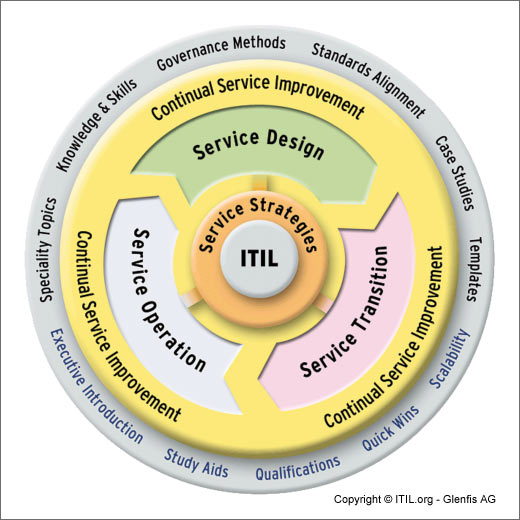
\includegraphics[width=0.50\textwidth]{Abbildungen/ITIL_Lebenszyklus}
	\caption[ITIL Service Lifecycle]{ITIL Service Lifecycle, Quelle: \url{http://os.itil.org/osMedia/site/t1 
	media/JPEG/01_itil_imap.jpg}}
	\label{fig:ITIL_Lebenyzyklus}
\end{figure}

\noindent
Es ist nicht notwendig, auf alle Teilbereiche einzugehen. Der Service Desk ist nämlich Bestandteil der Service Operation und somit die richtige Anlaufstelle für die Begriffsklärung. \newline \enquote{Service Operation beschreibt den Abschnitt des Lebenszyklus, der von den Kunden primär wahrgenommen wird.}\footnote{\citeauthor{Ebel} (\citeyear{Ebel}), S. 439.} In der Service Operations-Phase werden die Prozesse und Funktionen beschrieben, die einen stabilen  und bestmöglichen IT Service garantieren sollen. Bei dieser Verbindung von IT Organisation und Kunde wird besonders auf den Kunden eingegangen. Der Service Desk ist hierbei \enquote{die zentrale Anlaufstelle, der Single Point of Contact (SPoC) zwischen Anwender und der IT-Organisation}.\footnote{\citeauthor{Ebel} (\citeyear{Ebel}), S. 439.} Wie der Name schon verrät, kommt der Anwender nur über diese Schnittstelle in Kontakt mit der IT. Hier werden Meldungen der Anwender üblicherweise erfasst, kategorisiert und eingetragen. Der Service Desk ist nicht nur eine Kommunikationsunterstützung, sondern bietet gleichzeitig eine Auskunft für bereits bekannte Probleme. Dadurch kann bei häufig auftretenden Service-Unterbrechungen schneller gehandelt werden. Auch Supportanfragen, Beschwerden, Verbesserungsvorschläge oder Änderungswünsche können in den Service Desk eingetragen werden. Der Service Desk fungiert dadurch als sogenannter \enquote{Single Point of Contact}. Die nachfolgende Abbildung macht deutlich, dass der Kunde (Anwender) eine einzige Anlaufstelle hat, um seine Anliegen dem Support mitzuteilen. 

\begin{figure}[h!]
\centering
	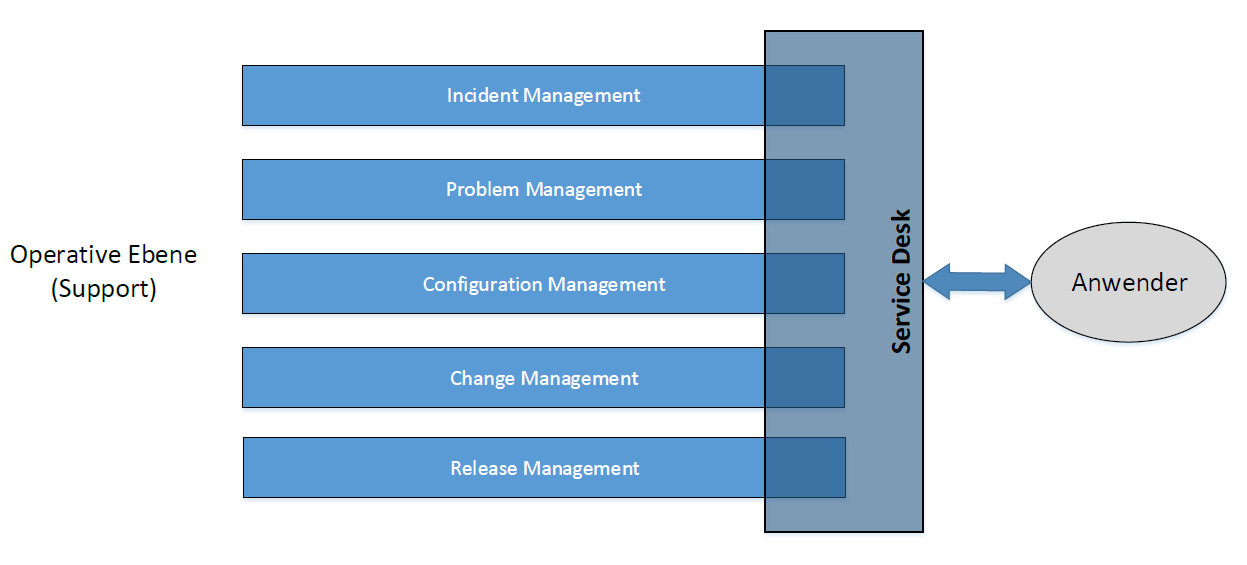
\includegraphics[width=0.70\textwidth]{Abbildungen/SPOC_4.png}
	\caption[Single Point of Contact]{Single Point of Contact, Quelle:http://edoc.hu-berlin.de/
	conferences/dfn2006/fischlin-roger-105/PDF/fischlin.pdf}
	\label{fig:ITIL_Single_Point_of_Contact}
\end{figure}

\noindent
Der Support kann die Meldungen der Anwender nun den entsprechenden Managementbereichen zuordnen. Eine Störmeldung von einem technischen Gerät würde beispielsweise zum Incident Management gehören. Ein Feature-Wunsch ist eher dem Teilbereich Change Management einzuordnen. Der Single Point of Contact  erleichtert so die Kommunikation zwischen dem Anwender und dem Support.\footnote{Vgl. \citeauthor{Ebel} (\citeyear{Ebel}), S. 65 ff.}\\ 


\subsection{Unterschied zu Help Desk}
\noindent
Bei der Begriffsabgrenzung zwischen Help Desk und Service Desk ist Vorsicht geboten. In mehreren Quellen ist zu finden, dass Help Desk (auch User-Help-Desk) lediglich ein veralteter Begriff für den Service Desk sei.\footnote{Vgl. \citeauthor{Buchsein} (\citeyear{Buchsein}), S. 26.}\footnote{Vgl. \citeauthor{Meier} (\citeyear{Meier}), S. 26.} Im Internet heißt es beispielsweise auf Wikipedia: \enquote{Die Artikel Helpdesk und Servicedesk überschneiden sich thematisch.}\footnote{Website: \citeauthor{WikiServiceDesk} (abgerufen am: 24.05.2016)} In anderen Literaturquellen tritt der Begriff Help Desk erst gar nicht auf oder wird dem Service Desk gleichgesetzt.\footnote{Vgl. \citeauthor{Olbrich} (\citeyear{Olbrich}), S. 19.} Im Zweifelsfall sollte man sich direkt auf das Buch ITIL Service Operation beziehen. In dem heißt es übersetzt unter dem Stichwort Help Desk:
\enquote{Eine Anlaufstelle für Anwender, um Incidents zu erfassen. Ein Help Desk ist in der
Regel eher technisch orientiert als ein Service Desk und stellt keinen Single Point
of Contact für die gesamte Interaktion bereit. Der Begriff 'Help Desk' wird häufig
auch als Synonym für Service Desk verwendet.}\footnote{\citeauthor{Cannon} (\citeyear{Cannon}), S. 233. Übersetzung entnommen aus: Ebel, N. (2008) S. 699.} \newline
In den weiteren Ausführungen gilt deshalb der Help Desk als Synonym für den Service Desk.

\newpage


\subsection{Aufgaben eines Service Desk}
\noindent
Im Folgenden sollen die wichtigsten Aufgaben eines Service Desk aus Sicht der ITIL v3 betrachtet werden. Hierfür wird zunächst stichpunktartig die Kernaussage festgehalten, um sie anschließend zu erläutern. Dabei beziehen sich die Kernaussagen auf die Ausarbeitung Olbrichs aus \enquote{ITIL Kompakt und verständlich}\footnote{\citeauthor{Olbrich} (\citeyear{Olbrich}), S. 19f.}
und sind eine leicht abgewandelte Form vom ITIL v3 Band Service Operation.\footnote{Vgl. \citeauthor{Cannon} (\citeyear{Cannon}), S. 110.}

\begin{itemize}
\item \enquote{Einheitlichen, zentralen Kommunikationsschnittstelle (SPoC) mit konkreten Ansprechpartner}
\end{itemize}
\noindent
Der Kunde hat mehrere Möglichkeiten, den Support zu kontaktieren. Schreibt der Kunde eine E-Mail an den Support, könnte diese ausgewertet und im Service Desk eingetragen werden. Ebenso könnte er selbst einen Eintrag über ein Web-Frontend erstellen. Oder aber der Support erstellt einen solchen Eintrag im Service Desk, wenn der Kunde zum Telefon greift. Es ist jedoch Voraussetzung, dass eine einheitliche und zentrale Kommunikationsschnittstelle bereitgestellt wird.


\begin{itemize}
\item \enquote{Aufnahme, Dokumentation und Auswertung aller Vorfälle}
\end{itemize}
\noindent
Wenn alle Vorfälle ordnungsgemäß aufgenommen und dokumentiert wurden, kann schneller reagiert werden, wenn sich ein Problem wiederholt. Dass alle Vorfälle auch ausgewertet werden sollten, ist verständlich und kann eventuell dazu beitragen, Folgeprobleme frühzeitig zu erkennen.

\begin{itemize}
\item \enquote{Überwachung, Nachverfolgung und Eskalation von laufenden
Supportvorgängen. Frühzeitiges Erkennen von
Bedürfnissen und Problemsituationen}
\end{itemize}
\noindent
Wie im Punkt zuvor erwähnt, können Probleme frühzeitig erkannt werden, indem Vorfälle genauestens ausgewertet werden. Das ist aber längst nicht die einzige Möglichkeit, Bedürfnisse der Kunden zu erkennen. Gute Mittel für vorausschauende Handlungen sind  bspw. Monitoring-Systeme oder Log-Files. Sie liefern technische Informationen, die - nach einer Auswertung - Aufschluss über die aktuelle Lage des Kunden geben und in den Service Desk integriert werden könnten. Nach ITIL v3 gibt es zwei Arten von Eskalation. Die funktionale Eskalation, bei der ein besonders schweres Problem oder die vergangene Zeit ein Auslöser wie die Eskalation eines Incidents ist. Im Gegensatz dazu ist bei hierarchische Eskalation eine Weiterleitung des Problems an die nächst höhere Eskalationshierarchie vorgesehen. Sollte beispielsweise ein Problem im Service Desk längere Zeit nicht bearbeitet und somit kein Fortschritt erzielt werden, eskaliert das Problem und wird entsprechend weitergeleitet\footnote{Vgl. \citeauthor{ITILBuch} (\citeyear{Victor}), S. 80f.}\footnote{Vgl. \citeauthor{Victor} (\citeyear{Victor}), S. 26ff.}


\begin{itemize}
\item \enquote{Überprüfung der Einhaltung des Dienstleistungsgegenstands
anhand von Service-Level-Agreements}
\end{itemize}
\noindent
Mithilfe des Service Desks kann kontrolliert werden, ob die vereinbarten Leistungen zwischen Auftraggeber und Beauftragten eingehalten wurden, wenn alle Vorfälle dokumentiert wurden.

\begin{itemize}
\item \enquote{Reporting – Beauskunftung gegenüber den Usern (Kunden)
und dem Management. Informationen über den aktuellen
Status von Vorgängen, geplanten Änderungen und
verschiedenen Nutzungsmöglichkeiten}
\end{itemize}
\noindent
Der Service Desk dient außerdem dazu, stets mit dem Kunden im Kontakt zu stehen. So können Informationen an den Kunden weitergeleitet oder auf der anderen Seite aktuelle Vorgänge, Status etc. des Kunden verfolgt und analysiert werden. 

\begin{itemize}
\item \enquote{Überprüfen der Kundenzufriedenheit, Stärkung der Kundenbeziehung.
Kontaktpflege. Aufspüren neuer Geschäftschancen}
\end{itemize}
\noindent
Nicht zuletzt kann der Service Desk auch als Instrument für einen ständigen Kontakt zum Kunden eingesetzt werden. Der Kunde hat dadurch den Eindruck, permanent mit der Support und somit der Firma verbunden zu sein. Das kann das Verhältnis zum Kunden stärken oder gar neue Geschäftsmöglichkeiten eröffnen.\\\\



\subsection{Nachteile ohne Servie Desk}
\noindent
Die vielseitigen Aufgaben eines Service Desk machen deutlich, welche Nachteile ein nicht vorhandener Service Desk für ein Unternehmen haben kann. Benutzer wissen bei Problemfällen nicht sofort, wer für die Bearbeitung des Vorfalls zuständig ist. Auch ist der Melder beispielsweise für eine Störmeldung nicht sofort identifizierbar. Rückfragen sind daher schwer möglich und die gesamte Bearbeitung des Problems verzögert sich stark.\\

\noindent 
Bei der Erfassung von Vorfallen sind im Service Desk bestimmte Informationen nötig, die normalerweise über ein Formular o.ä. erfasst werden. Wenn der Service Desk - und damit auch ein Formular zu Erfassung - komplett fehlt, kann es zu unvollständigen Vorfallbeschreibungen kommen. Auch hier wird der Prozess für die Problembehandlung verlangsamt.\\

\noindent
Probleme, die häufig auftreten, werden nur teilweise bis gar nicht dokumentiert. Dadurch werden immer wieder neue Lösungsansätze gesucht, ohne auf bereits vorhandene und bewährte Lösungen zurückzugreifen. Eine Wissensdatenbank ist daher unmöglich.\\

\noindent
Das Anschaffen einer Service Desk-Lösung sowie die zugehörigen Schulungsausgaben sind natürlich mit Kosten verbunden, doch ein effektives Vorgehen beim Lösen eines Vorfalls mittels des Service Desks kann die Gesamtkosten reduzieren. Demzufolge würde ein gut implementierter Service Desk dazu beitragen, die Kosten insgesamt zu senken.\footnote{Vgl. \citeauthor{Olbrich} (\citeyear{Olbrich}), S. 26f.}\\

\noindent
Unter bestimmten Voraussetzungen ist es möglich, dass ein Kunde direkt mit dem Fachpersonal - beispielsweise aus der Entwicklungsabteilung - kommuniziert, anstatt mit einem Supportmitarbeiter. Das geschieht, wenn keine Filterung der eingetroffenen Probleme vorgenommen wird. Ein Entwickler könnte somit einem fragenden Kunden gegenüberstehen, dessen Problem eher in den Bereich Release Management einzuordnen ist. Ein Supportmitarbeiter wäre in diesem Fall der bessere Gesprächspartner für den Kunden.\\

\noindent
Der Kunde hat beim Fehlen eines Service Desk keinen Single Point of Contact mehr und könnte möglicherweise nicht wissen, an wen er sich bei Problemen zu wenden hat. Es fehlt ein wichtiger Kommunikationsweg, der nicht ohne weiteres ersetzt werden kann. Dadurch könnte auch die Beziehung zwischen dem Unternehmen und dem Kunden leiden.\\\\



\noindent
In diesem Punkt wurden die begrifflichen Grundlagen für das weitere Vorgehen gelegt. Es wurde deutlich gemacht, welche Aufgaben ein Service Desk hat und somit auch, wie wichtig er für die Kommunikationsstruktur eines Unternehmens sein kann. Nicht nur der Kontakt zum Kunden kann durch den Service Desk verbessert werden, auch das Protokollieren und Lösen von Problemen innerhalb einer Firma ist mit dem Service Desk besser zu bewältigen.\newline









   


 
	
\newpage


%-------------------------------------------------------------------------------------------------------
%					3	Analyse verschiedener Softwarelösungen
%-------------------------------------------------------------------------------------------------------

\section{Analyse verschiedener Service Desk-Lösungen}

\subsection{Schwerpunkte der Analyse und Ausgewählte Service Desk-Lösungen}

\noindent
Nach diesem sehr theoretischem Ansatz die Einsatzmöglichkeiten und Aufgaben eines Service Desks zu klären, werden nun Praxisbeispiele analysiert. Wichtig sind dabei nicht Kriterien wie das äußere Erscheinungsbild oder die Kosten. Ziel soll es sein durch einen Vergleich gängiger Softwarelösungen, Verbesserungsmöglichkeiten der eigenen Service Desk-Funktionalitäten in GEBman10 zu ermitteln. Dabei wird auf die drei folgenden Punkte Wert gelegt:

\begin{itemize}
\item Funktionalität:\\
		Die Funktionalität ist wohl das fundamentalste Kriterium. Hier ist entscheidend, welche 			
		Möglichkeiten dem Benutzer gegeben werden bspw. Meldungen/Tickets anzulegen, zu 
		zuweisen, zu suchen oder zu filtern. Wichtig ist aber auch, welche Informationen in welcher 
		Darstellungsform erhalten sind (Diagramme etc.) und welche Daten erfasst werden müssen 
		bzw. können.\\
		 
\item Bedienbarkeit:\\
		Aus diesem Blickwinkel ist es entscheidend, welche Bedienelemente vorhanden und wie diese angeordnet sind. Eine	
		Bewertung nach intuitiver Bedienbarkeit ist schwierig vorzunehmen, da das immer eine
		subjektive Ansicht enthält.\\
		
\item Anpassbarkeit:\\
		Inwieweit kann man bspw. die grafische Oberfläche vom Benutzer geändert und auf die 
		eigenen Bedürfnisse angepasst werden.\\		
\end{itemize}


\noindent
Nach den Recherchen auf mehreren Review und Ranking Websites zum Thema Service Desk / Help Desk, sind drei Softwarelösungen wiederholt erwähnt und gut bis sehr gut bewertet worden.\footnote{Website:\cite{Ranking1}}\footnote{Website:\cite{Ranking2}}\footnote{Website:\cite{Ranking3}}Diese drei webbasierten Anwendungen werden nun vorgestellt und anschließend ihre Stärken bzw. Besonderheiten dargelegt. Im Anhang auf Seite~\pageref{Anhang3} befindet sich jeweils ein Screenshot von jeder Softwarelösung.

\begin{itemize}
\item Freshdesk:\\
		Girish Mathrubootham beschloss 2010 nach dem Lesen eines Nachrichtenartikels die Firma 
		Freshdesk ins Leben zu rufen. Das gleichnamige Produkt wird laut eigenen Angaben von rund 
		70.000 Kunden aller Unternehmensgrößen genutzt.\footnote{Website:\cite{Freshdesk}}
		\\
		 
\item Desk.com:\\
		Das Unternehmen Salesforce.com legt laut eigenen Angaben großen Wert auf mobile 
		Endgeräte und soziale Netzwerke.\footnote{Website:\cite{Salesforce}}Die Service Desk -Lösung des 
		Unternehmens nennt sich 	Desk.com und zu ihren Kunden zählen unter anderem die Firma FlixBus und die 
		Commerzbank.
		\\
		
\item Zendesk:\\
		Zendesk beschreibt sich selbst als \enquote{Kundenservice-Plattform}. Die gleichnamigen 
		Firma hat nach eigenen Angaben mehr als 75 000 Unternehmen, die diese Plattform nutzen. 
		Entstanden ist das Unternehmen 2007 aus einer Idee von drei Freunden aus Kopenhagen.
		\footnote{Website:\cite{Zendesk}}
		\\		
\end{itemize}

\noindent
Aktuell benutzt der Support von der KMS Computer GmbH die Software SysAid für den Service Desk. Durch eine Vielzahl von Einträgen und Erfahrungen der Mitarbeiter im Support, ist es sinnvoll auch diese Anwendung mit in den Vergleich einfließen zu lassen.

\begin{itemize}
\item SysAid:\\
		 Die Help Desk-Software SysAid wird nach eigenen Angaben in über 10 000 Unternehmen in 
		 140 Ländern eingesetzt. Die Firma SysAid Technologies wurde 2002 gegründet und zählt somit 
		 zu den erfahrenden Unternehmen dieser Branche.\footnote{Website:\cite{SysAid}}
		\\\\
\end{itemize}	

\subsection{Freshdesk}
\noindent
Alle im Freshdesk angemeldeten Support Mitarbeiter werden als Agenten bezeichnet
Der Freshdesk besticht mit seinem sehr simplen Dashboard, was der Bedienbarkeit zugutekommt. Zur Erklärung: ein Dashboard ist üblicherweise eine kompakte meist grafisch aufbereitete Ansicht von Informationen. Der Agent erhält hier nur die wichtigsten bzw. neuesten Informationen. Auf den ersten Blick kann der Agent sehen, welche Tickets offen, nicht zugewiesen oder überfällig sind. Zusätzlich erhält der Agent die Möglichkeit, individuelle Aufgaben zu notieren und wie eine Checkliste abzuarbeiten. Ein sehr nützliches Feature für kleinere Notizen bzw. Probleme.\\ 
Erst im zweiten Menüpunkt kann der Agent Tickets filtern. Hierfür gibt es gängige auswählbare Filter oder die Option einen Filter selbst zu konfigurieren und zu speichern. Wählt der Agent hier nun ein oder mehrere Ticket aus, gelangt er in eine Detailansicht eines Tickets und kann dann zwischen den ausgewählten wechseln. In der Detailansicht kann er nun den gesamten Verlauf betrachten, auf das Ticket antworten, das Ticket weiterleiten etc. . Ein Seitenmenü ermöglicht die Einsicht auf die wichtigsten Informationen des Ticketerstellers. Außerdem können die Ticket-Eigenschaften in diesem Seitenmenü geändert und somit die Priorität und der Status festgelegt werden. Zusätzlich gibt es eine Typisierung des Tickets. Im Punkt 2.1 wurden die verschiedenen IT Service Managementbereiche dargelegt. Durch die Typisierung kann festgelegt werden, welchem Managementbereich das Ticket entspricht. Handelt es sich beispielsweise um einen Notfall, wird der Typ als Incident bestimmt und kann so bei der Suche schneller gefunden werden.\\
Ein weiterer Menüpunkt nennt sich \enquote{Soziales} und hat eine spezielle Funktionalität zu bieten. Freshdesk bieten nämlich die Möglichkeit, die Kunden über einen \enquote{sozialen Support} zu betreuen. Laut eigenen Angaben begründet Freshdesk den Kontakt mit Kunden über soziale Kanäle wie folgt: \enquote{Tatsächlich erwarten 32 \% der Kunden in sozialen Netzwerken eine Antwort auf Ihre Anfragen innerhalb von 30 Minuten.} Weiterhin heißt es, bei schnellen und effektiven Antworten würden 71\% der Kunden den Support weiterempfehlen. Wie Freshdesk zu diesen Zahlen kommt, bleibt zunächst unklar. Recherchiert man ein wenig im Netz, so kann man diese Zahlen in einem Bericht von t3n wiederfinden, der auf einer Studie von  Bain \& Company beruht.\footnote{\citeauthor{Rixecker}. Website:\cite{Rixecker}} Wichtiger als die Zahlen ist jedoch die Idee, über soziale Netzwerke mit dem Kunden zu interagieren und somit eine teils freundschaftliche Beziehung aufzubauen. Erlaubt man Freshdesk im Administrator-Bereich, sich über ein Twitter-Konto einzuloggen, so kann direkt im Service Desk auf Twitter zugegriffen werden. Auch eine Facebook-Seite kann in den Service Desk von Freshdesk integriert werden. Diese Funktionalität wirkt sehr modern und bietet neue Ansatzpunkte in der Kundenbetreuung.\\
Im dritten Menüpunkt erhält der Agent die Option eine Knowledge Base anzulegen. Diese Wissensdatenbank kann direkt vom Kunden aufgerufen werde, um eine erste Hilfestellung bei bekannten Problemen zu erhalten. Mit Kategorien wie Frequently Asked Questions (FAQs) kann die Wissensdatenbank unterteilt werden und bietet dem Kunden so eine gute Übersicht.\\
Auch ein Forum kann mit dem Freshdesk gepflegt werden. Im Unterpunkt Foren können mehrere Foren verwaltet werden und Themen wie \enquote{Tips und Tricks} oder \enquote{Wie erstelle ich ein Ticket?} dem Kunden ein optimales Handbuch oder Nachschlagewerk liefern.\\
Des Weiteren kann im Menüpunkt Berichte auf umfassende Analysen Einsicht genommen werden. Nicht nur wie lange ein Ticket durchschnittlich bearbeitet wurde ist in Diagrammen dargestellt, sondern auch wie viele Tickets die Kunden aufgegeben haben oder wie viel Tickets ein Agent schon bearbeitet hat. Trotz der großen Informationswiedergabe bleibt Freshdesk übersichtlich und gut strukturiert. Die Berichte kann sich der Agent auch per Mail in Form einer PDF - oder CSV-Datei zuschicken lassen.\\
Der bereits erwähnte Administrator-Bereich kann sehr gut genutzt werden, um den Service Desk anzupassen. Von allgemeinen Einstellungen wie den Feldern, die bei der Ticketerstellung ausgefüllt werden müssen, bis zu dem Import von Daten aus anderen Service Desk-Lösungen kann der Freshdesk sehr gut and die Bedürfnisse der Agents oder Gruppen von Agents angepasst werden.\\
Egal in welchem Menüpunkt der Agent sich bewegt, es stehen ihm immer ein Button für das Anlegen eines neuen Tickets und einer Suche in der oberhalb liegenden Menüleiste zur Verfügung. Der Freshdesk ist somit ein in sich schlüssiges System mit vielen modernen und anschaulichen Extras.\\

\subsection{Desk.com}
\noindent
Desk.com ist eine Service Desk-Lösungen, die besonderen Wert auf den mobilen Einsatz des Supports legt. Das spiegelt sich auch in der Desktop Webanwendung wieder. Die Oberfläche erinnert stark an eine App auf einen mobilen Endgerät. Die Benutzer werden in Desk.com ebenfalls Agents genannt. 
Eine statische Menüleiste ist auch hier oberhalb der Ansicht zu finden. Hier befinden sich große Buttons für das Anlegen eines neuen Tickets, eine Suche, ein Button für weitere Menüs und eine Art Tab-Ansicht der neusten Tickets. Das Dashboard besteht aus eine Auflistung aller Tickets, die nur die nötigsten Informationen liefern. Spalten können sich aber noch zusätzlich einblenden lassen. Filtern lassen sich die Tickets an dieser Stelle mit einer Auswahl auf der linken Seite. Jedoch ist diese Auswahl sehr eingeschränkt auf alle Tickets oder Tickets, die dem Agent zugewiesen wurden. Eine Hoverbox ermöglicht die Einsicht der Beschreibung des Tickets, ohne dieses öffnen zu müssen. Hierfür muss der Agent lediglich den Mauszeiger über das Ticket halten und nach wenigen Sekunden erscheint eine kleines Fenster. Die Service Desk-Lösung von Desk.com hat ebenfalls einen eigenen Menüpunkt für die Einsicht von Berichten. Nicht ganz so umfangreich wie beim Freshdesk, aber dennoch anschaulich in Diagrammen dargestellt. Die Funktionalität einer Wissensdatenbank bietet der Desk.com ebenso. Allerdings kann diese nur im Administrator-Bereich verwaltet und erweitert werden.\\
Insgesamt wirkt der Desk.com maßgeschneidert für mobile Endgeräte. Und genau hier liegen auch die Stärken der Service Desk-Lösung. Durch die großen Bedienelemente und stark vereinfachten Ansichten, wird das Arbeiten auf Tablet o.ä. deutlich erleichtert. Für eine Desktop Variante nicht unbedingt die beste Wahl, auch weil sich der Service Desk - wenn überhaupt - nur sehr umständlich auf die individuellen Bedürfnisse anpassen  lässt. Für Mitarbeiter, die ständig unterwegs sind, ist das System durchaus attraktiv.\\

\subsection{Zendesk}
\noindent 
Der Zendesk hat seine Stärken in den umfassenden Hilfestellungen für die Agents. Schon im Dashboard erhält ein Agent eine knappe aber präzise Erklärung der einzelnen Teilbereiche des Service Desk. Zunächst muss der Agent die einzelnen Kanäle wie E-Mail oder Telefon einrichten. Auch im Zendesk sind  Twitter und Facebook als Kommunikationswege denkbar. In fast allen Einrichtungsschritten wird der Agent mit Anweisungen unterstützt und kann sich direkt im Zendesk ein Video-Tutorial anschauen.\\
Eine statische Leiste befindet sich im Zendesk oberhalb mit einer Suchfunktion und er Möglichkeit neue Tickets zu erstellen. Ein ebenfalls festes Menü am Seitenrand hat nur die wichtigsten Unterpunkte: Dashboard, Tickets , Berichte und Einstellungen. Eine Anordnung, die bereits aus den anderen Service Desk-Lösungen bekannt ist. Das Menü kann angepasst werden, wenn alle Kanäle eingerichtet sind.\\
Neben den bereits bekannten Features von den andern Softwarelösungen, bietet Zendesk weitere Funktionalitäten. Durch eine große Auswahl an Apps kann der Service Desk ganz nach eigenen Vorstellungen des Agents angepasst werden. Ein einfaches Beispiel hierfür ist das Anzeigen von Kontaktinformationen direkt neben einem Ticket. Die App trägt den schlichte Namen Benutzerdaten. Wurde diese Erweiterung erfolgreich installiert, kann der Agent über einen Button die Funktionalitäten der Apps bei der Ticketübersicht nutzen,  um weitere Informationen über den Kunden zu gewinnen. Dabei besteht die Möglichkeit Notizen oder Details über den Kunden in der App einzutragen.\\
Über ein Web Widget ist es möglich, auf Komponenten von Zendesk wie die Wissensdatenbank oder Live-Chat zu zugreifen. Als Widget bezeichnet man einfache kleine clientseitige Programme, die durch minimalem Eingabeaufwand zusätzliche Funktionen oder Informationen bereitstellen.\footnote{Website:\cite{Widget1}} \footnote{Website:\cite{Widget2}} Dieses Web Widget kann in Webseiten eingebettet werden, in dem in den Einstellungen das Widget aktiviert und auf der Webseite der Source-Code eingebunden wird. Eine Funktionalität die vor allem bei Unternehmenswebseiten  eingebaut werden könnte.\\
Um festzustellen, wie sehr die Kunden mit dem Service Desk zufrieden sind, kann mit dem Zendesk eine Kundenumfrage gestartet werden. Die Fragen hierfür lassen sich allerdings nicht konfigurieren. Der Kunde kann (bei aktivierter Option) auch die Tickets bewerten und somit ebenfalls Feedback für den Agent geben.\\
Zendesk bietet eine Vielzahl von Funktionalitäten, die sowohl neue Kommunikationsmöglichkeiten mit dem Kunden garantieren, als auch die Bedienung des Service Desk für die Agents erleichtern. Es ist aber anzumerken, dass es durchaus eine gewisse Zeit in Anspruch nimmt, alle Features einzurichten und richtig zu bedienen. Einsteiger Agents sollten deshalb gut geschult werden.\\

\subsection{SysAid}
\noindent
Da diese Bachelorarbeit in einem knappen Zeitrahmen fertiggestellt werden muss, konnten keine ausführlichen Betrachtungen der Service Desk-Lösungen durchgeführt werden, wenn diese mit vielen Daten gefüllt sind. Hierzu wären mehrere Kontaktinformationen und Ticket-Erstellungen nötig. Deshalb wird nun der firmeneigene Support nach Besonderheiten in der Softwarelösung SysAid befragt. Bei täglichem Gebrauch kommen unvorhersehbare Situationen zustande, die kaum in der Vorbetrachtung zu erahnen sind. Daher ist die Betrachtung vom SysAid der KMS Computer GmbH eine sinnvolle Vorgehensweise bei der Ermittlung von Verbesserungsmöglichkeiten im Bereich Service Desk-Anwendungen.\\
\noindent
Die Startseite von SysAid wirkt nicht besonders aussagekräftig. Dem Benutzer werden mehrere Fenster angezeigt, die nur sehr wenige und auch nur allgemeine Information über aktuelle Tickets enthalten. Um zu der Übersicht der Tickets zu gelangen, muss erst in den Menüpunkt Service Desk gewechselt werden. Hier sind nun alle Tickets mit einer ID gelistet und wirken sehr strukturiert. \newline
SysAid verfügt auch über eine Wissensdatenbank, die vom Support angepasst werden kann. Die Anzeigefenster sind allerdings sehr klein gehalten und lassen sich in ihrer Größe nicht anpassen. Für einen Kunden wirkt die Wissensdatenbank deshalb nicht sehr ansprechend.\newline
Als eine Stärke von SysAid ist die Erinnerung an eskalierte Tickets zu nennen. Wenn ein Ticket über eine einstellbares Intervall  nicht bearbeitet wurde oder schon seid längerer Zeit im Status \enquote{in Bearbeitung} verharrt, eskaliert das Ticket.\newline
Durch diese Funktion wird ein Support-Mitarbeiter daran erinnert, wenn sich bei einem Ticket keine Veränderung zeigt. Hier sollte dann mit Nachdruck auf die Lösung hingearbeitet werden. Eine weitere Stärke von SysAid ist die Möglichkeit, das Problem eines Tickets direkt in Wissensdatenbank aufzunehmen. Das erleichtert das Erstellen eines Eintrags in die Wissensdatenbank. \newline
Das System erkennt  gleiche Absender nicht und alle Tickets kommen daher in einziges Sammelbecken. Das macht eine Zuordnung schwierig, ist aber mit einer Eintragung übergeordneter ID's manuell möglich.\newline
Beim Erstellen eines Tickets ist es wie bei Zendesk und Desk.com nicht möglich, Bilder direkt in den Text einzufügen. Durch das anhängen von Screenshots o.ä. geht nach dem Support der direkte Bezug zwischen Beschreibung des Problems und der Verdeutlichung mit Hilfe eines Bilds verloren.\newline
Der Support gab an, das die Wissensdatenbank von Kunden kaum genutzt wird. Das liegt wohl daran, dass sich die Kunden in SysAid nicht einloggen. Es werden auch wenige Tickets direkt über SysAid erstellt, sondern über die E-Mail Integration.\newline
Der Administrationsbereich von SysAid bietet die Möglichkeit, die Benutzeroberfläche umfassend anzupassen. Dadurch können nicht gebrauchte Informationen ausgeblendet werden und die Benutzeroberfläche für den Support-Mitarbeiter auf das nötigste reduzieren. Des Weiteren können die Betriebszeiten des Help Desks eingestellt werden, was sinnvoll für die Eskalation von Meldung ist\newline
Es fällt auf, dass die Alarme in SysAid nur begrenzt konfigurierbar sind. Es sind lediglich vier Alarmstufen bzw. Status die man damit abdecken kann, was von den Mitarbeitern des Supports bemängelt wird. Auch eine grafische Auswertung fehlt in der Version, die der Support von der KMS Computer GmbH zur Verfügung hat. Es gibt aber die Option, Reports in Form von Excel - oder PDF-Dateien erstellen zu lassen.

\subsection{Fazit der Analyse}

\noindent
Die Service Desk-Lösungen werden nun nach den in Punkt 3.1 genannten Kriterien bewertet. Die Tabelle~\ref{tab:Auswertung} stellt das Ergebnis dar. Jedes der Kriterien kann mit maximal 10 Punkten bewertet werden. Die Funktionalität hat die höchste Gewichtung, gefolgt von der Bedienbarkeit und der Anpassbarkeit. Die Gewichtungen stehen hinter den Kriterien Klammern. Die Gesamtpunktzahl findet sich in der letzten Tabellenzeile wieder.\\

\begin{table}[h!]
    \begin{tabular}{ | p{3.5cm}| p{2.5cm} | p{2.5cm} | p{2.5cm} | p{2.5cm} |}
    \hline
       & Freshdesk & Desk.com & Zendesk & SysAid \\ \hline
   Funktionalität (5) & 9 & 6 & 8,5 & 8 \\ \hline
   Bedienbarkeit (3) & 9 & 8 & 9 & 6,5 \\ \hline
   Anpassbarkeit (2) & 7,5 & 5 & 7,5 & 6 \\ \hline
   Gesamtpunktzahl & 87 & 64 & 84,5 & 71,5 \\ \hline
    \end{tabular}
    \caption[Bewertung der Service Desk-Lösungen]{Bewertung der Service Desk-Lösungen, Quelle: eigene Darstellung}
    \label{tab:Auswertung}
\end{table}

\noindent
Die Lösung von Freshdesk und Zendesk überzeugten am meisten. Aufgrund des großen Funktionalitätsumfangs und guter Bedienbarkeit erhielten sie fast die höchste Punktzahl in diesen Bereichen. Nur bei der Anpassbarkeit - gerade in der Gestaltung der Bedienoberfläche - mussten kleine Abstriche gemacht werden.\newline
Desk.com stach weder bei den Funktionalitäten, noch in der Anpassbarkeit heraus und konnte sich deshalb auch in der Punktetabelle nicht durchsetzen. Lediglich bei der schlicht gehaltenen Bedienung gab es Punkte.\newline
SysAid befindet sich im Mittelfeld der Punktetabelle, da die Funktionalitäten gut sind, die Softwarelösung aber in der Bedienbarkeit und Anpassbarkeit nicht überzeugen konnte.\\


\noindent
Alle Service Desk-Systeme, die betrachtet wurden, waren auf ihre Weise individuell. Die Schwerpunkte waren unterschiedlich gelegt und einen \enquote{Sieger} der Analyse zu bestimmen wäre daher nicht sinnvoll. Wichtiger ist viel mehr, wie die Stärken der Systeme möglicherweise Anreize für Verbesserungen der Service Desk-Lösungen in GEBman 10 bieten.\\

\noindent
Der Freshdesk hat seine Stärken klar in der grafischen Aufbereitung der erfassten Daten und in der Einbindung von sozialen Medien. Auch wirkte diese Service Desk-Lösung sehr übersichtlich in allen Teilbereichen. Das lag nicht zuletzt an der Beschränkung auf die wichtigsten Information im jeweiligen Menüpunkt. Bilder konnten direkt in der Ticket-Beschreibung eingefügt werden, um somit einen direkten Bezug zu der Vorfallbeschreibung herstellen zu können.
\newline
Desk.com konnte besonders im mobilen Bereich überzeugen. Die Bedienelemente wurden eher schlicht gehalten und das System bietet Funktionalitäten im richtigen Maße für mobile Einsätze. Das könnte für die KMS Computer GmbH interessant werden, da der mobile Ausbau von GEBman10 im vollem Gange ist und ein Service Desk Modul noch nicht umgesetzt wurde. \newline
Als Stärke des Zendesk sind die guten und ausführlichen Hilfestellungen für die Benutzer (Agents) zu nennen. Besonders für Einsteiger dürfte das eine große Erleichterung in der Einarbeitung sein. Zudem kann der Zendesk sehr einfach erweitert und somit auf individuelle Einsatzbereiche angepasst werden. \newline
Bei der Service Desk-Lösung SysAid wurde die Eskalation von Tickets und die damit einhergehende Erinnerung an den Support-Mitarbeiter als vorteilhaft im Arbeitsalltag benannt. Sollte doch einmal eine Meldung in Vergessenheit geraten, kann dem durch diese Sicherheitsmaßnahme entgegen gewirkt werden.\\\\

\noindent
Es lassen sich aber auch Gemeinsamkeiten benennen, die sich in allen Systemen in leicht abgewandelter Form wiederfanden und die somit einen besonderen Stellenwert besitzen:

\begin{itemize}
\item Menüleiste ermöglichte es dem Agent/Benutzer jederzeit zu suchen und ein neues Ticket anzulegen.
		 
\item durch farbliche Kennzeichnung waren die Status der Tickets sofort einsehbar
		
\item  Kontaktdaten vom Kunden in der Detailansicht eines Tickets

\item Filtereinstellungen für Tickets konfigurierbar und speicherbar

\item alle Berichte/grafischen Auswertungen in einem Extramenüpunkt.

\item Erstellung und Verwaltung einer Wissensdatenbank möglich
\end{itemize}

\noindent
Dieses Fazit der Analyse der verschiedenen Service Desk-Lösungen kann dazu genutzt werden, Verbesserungsmöglichkeiten im Service Desk Modul von GEBman 10 zu  bestimmen. 
	
\newpage


%-------------------------------------------------------------------------------------------------------
%					4	Service Desk in GEBman10
%-------------------------------------------------------------------------------------------------------

% !TEX root = Bachelorarbeit_Paul_Zilewitsch.tex

\section{Der Service Desk in GEBman 10}

\subsection{Aktuelle Umsetzung}
\noindent
Zunächst ist anzumerken, dass sich das Service Desk Modul stark an den anderen Modulen in GEBman 10 orientiert und an sie gebunden ist. Das unterscheidet sich deshalb sehr stark von den zuvor betrachteten Service Desk-Lösungen und wurde bisher nur im Bereich Facility Management eingesetzt. Aus diesem Grund ist es nur bis zu einem gewissen Grad möglich, diese Lösung in GEBman 10 mit anderen Service Desk-Softwarelösungen zu vergleichen. Ihre Aufgabenfelder und Schwerpunkte schlicht zu unterschiedlich sind. Dennoch ist es möglich, Verbesserungsmöglichkeiten zu identifiziert, welche das Service Desk Modul auch außerhalb des Facility Management Bereiches einsetzbar machen können. Hierzu wird zunächst die aktuelle Umsetzung von dem Service Desk in GEBman10 festgehalten.\\

\noindent
Der Service Desk  ist ein eigenständiges Modul, welches standardmäßig in jeder Version von GEBman 10 enthalten ist. Es dient in erster Linie dazu, unvorhergesehene Störungen für Geräte, Gebäude, Inventare, Fahrzeuge, Bäume, Grünflächen und Beleuchtungseinheiten erfassen zu können. Aus diesem Grund ist das Modul stark an andere Module gebunden und legt die Schwerpunkte auf den Bereich Facility Management. Das Modul kann aber auch für eine Service Desk-Lösung für das Unternehmen verwendet werden. Hierzu müssen lediglich alle Mitarbeiter einen Account anlegen, um so als Melder agieren oder als Bearbeiter reagieren zu können.\\

\noindent 
Die Bedienoberfläche ist in einzelne Sektionen unterteilt. Im Dashboard dieses Moduls werden alle Meldungen in einer Sektion angezeigt, die erstellt wurden. Alle Meldungen haben eine eindeutige Nummer (Identifikator). Rechts daneben wird der Standort des Objektes angezeigt, für das die Meldung aufgegeben wurde. Es werden auch bereits abgeschlossene bzw. erledigte Meldungen angezeigt. Der Benutzer erhält mittels eines Berichtes in Diagrammform in einer weiteren Sektion direkt einen Einblick auf die Meldungen innerhalb einer Woche. Unterteilt wird hierbei in eingegangene Meldungen, Meldungen, die in Bearbeitung sind, unbearbeitete Meldungen und fertige Meldungen. Ein weiterer Bericht veranschaulicht die Verweildauer einer Meldung, in dem die Zeit zwischen dem unbearbeiteten Zustand und dem der Bearbeitung protokolliert wird. Unter den beiden Diagrammen finden sich alle Fakten noch einmal in Form von Zahlen wieder. Es ist derzeit noch nicht Möglich, diese Berichte/Diagramme individuell anzupassen. Der Aufbau wird in der Abbildung~\ref{fig:GEBman10 Service Desk Dashboard} deutlicher. \\ 

\begin{figure}[h!]
\centering
	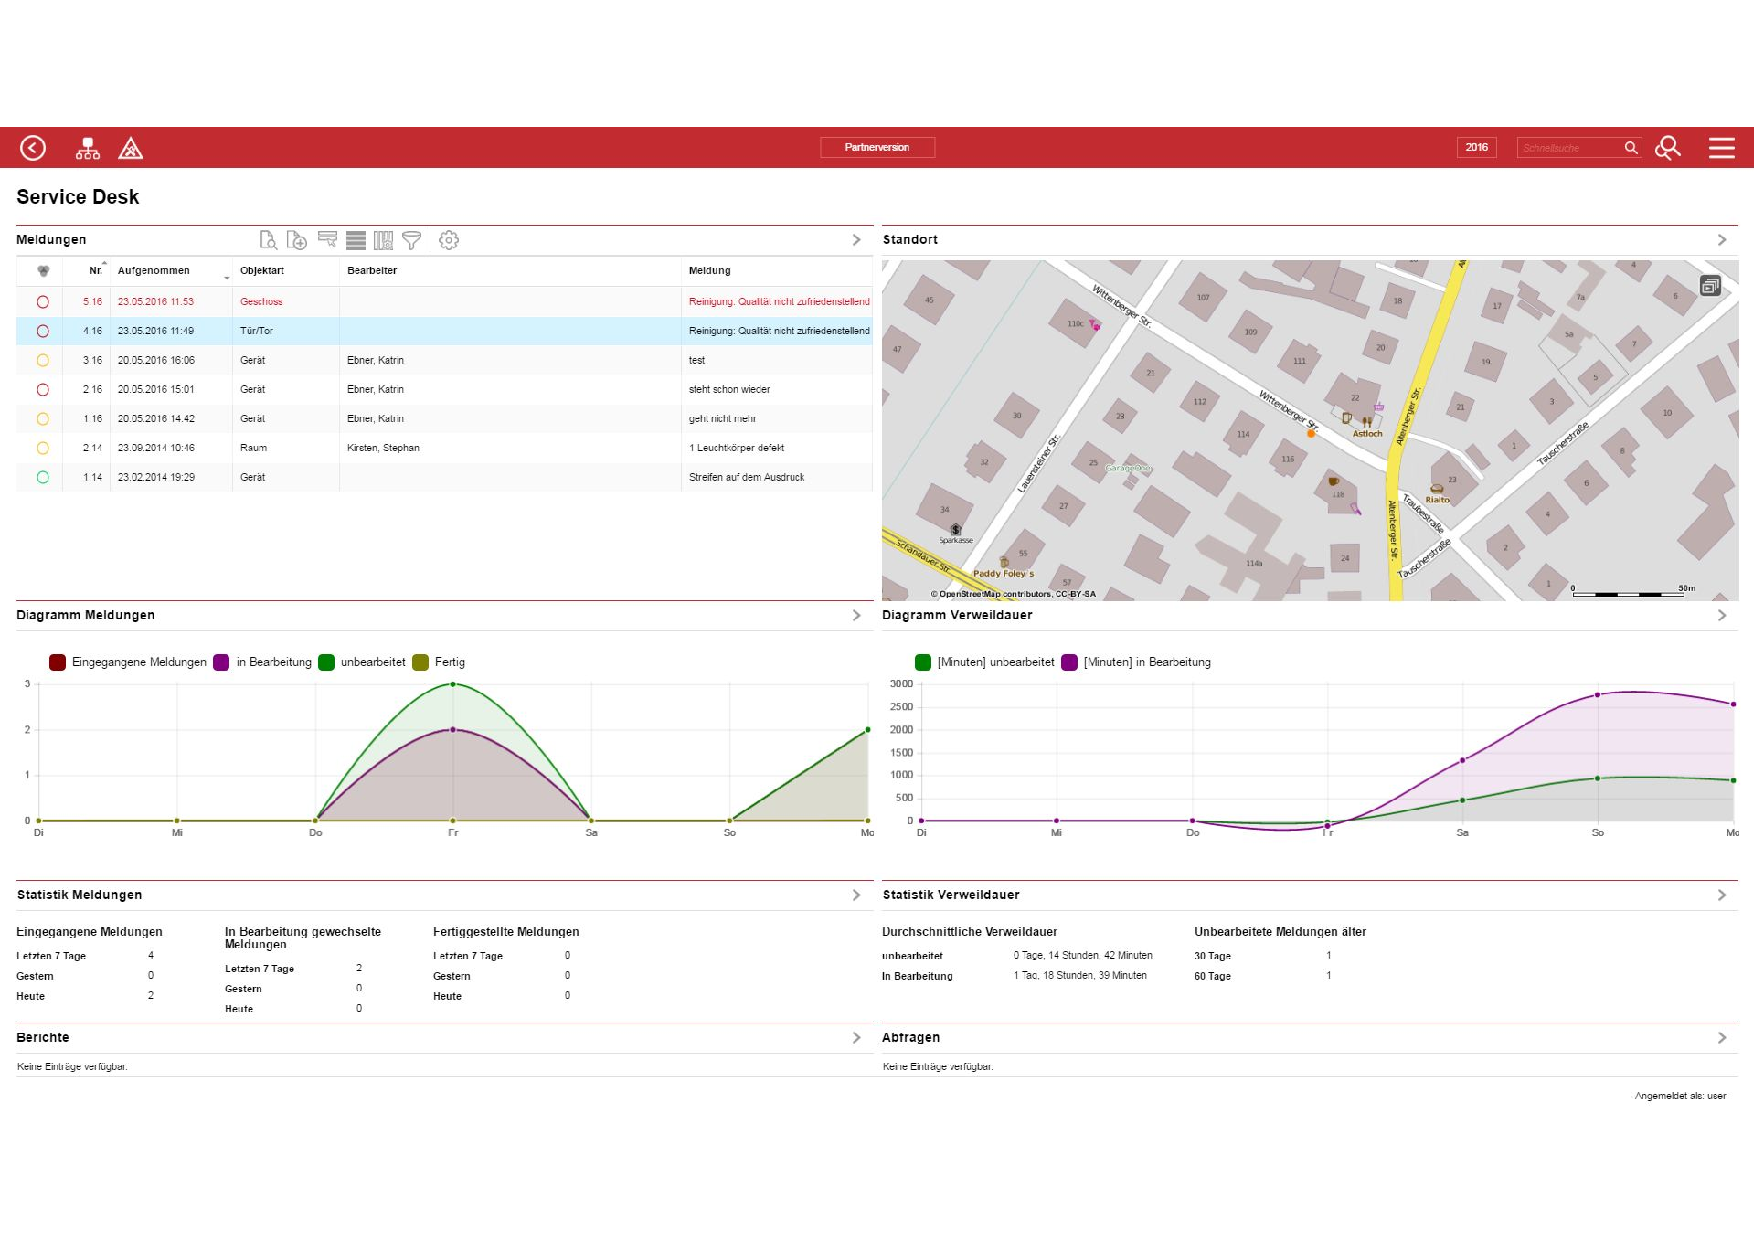
\includegraphics[width=0.75\textwidth]{Abbildungen/GEBman.png}
	\caption[GEBman 10 Service Desk Dashboard]{GEBman 10 Service Desk Dashboard, Quelle: 
	GEBman 10}
	\label{fig:GEBman10 Service Desk Dashboard}
\end{figure}

\noindent
Der Benutzer hat im Dashboard die Möglichkeit für eine direkte Detailansicht einer oder mehrerer Meldungen, eine neue Meldung anzulegen, eine Filterung der Meldung vorzunehmen oder die Einstellungen anzupassen. Bei den Einstellungen kann entschieden werden, an welchen Positionen die Sektionen der Bedienoberfläche verankert werden sollen.\newline
Die Speicherung der Filter ist in der Dashboard-Ansicht des Service Desk Moduls nicht möglich. Hierfür muss der Benutzer in der Suchliste eine Abfrage definieren und diese abspeichern. Außerdem ermöglicht die Suchliste eine detailliertere Filterung, einen Excel Export, das Löschen von Meldungen und die Generierung von Maßnahmen. Das Generieren von Maßnahmen ist eine zentrale Funktionalität im Service Desk. Manche Vorfälle lassen sich nicht ohne Fachpersonal bewältigen. Hierfür müssen unter Umständen spezielle Mitarbeiter oder eine andere Firma angefordert werden. Mit der Maßnahmengenerierung kann ein Auftrag für den Mitarbeiter bzw. die Firma erstellt werden. Wenn sich eine andere Firma um die Maßnahme für den Vorfall kümmert, wird das am Objekt in der Sektion Fremdvergabe angezeigt. \newline
Bevor man den Service Desk nutzt, ist es sinnvoll, die drei Standardkataloge für den Service Desk zu bearbeiten. Mit Katalogen können in GEBman 10  vorgefertigte Auswahlmöglichkeiten erstellt werden, die später im entsprechenden Modul zur Anwendung kommen. Dem Service Desk stehen folgende Kataloge zur Verfügung:\\

\begin{itemize}[itemsep=10pt]
\item Art:\\
		Mit der Art ist in diesem Fall die Meldungsart gemeint. Dem Benutzer steht frei, welche 
		Meldungsarten er hier definiert, um auch die ausgefallensten Vorfälle möglichst präzise beschreiben zu 
		können.  \\
		 
\item Meldungsvorlage:\\
		Nicht selten ähneln sich Meldungen, da sich Vorfälle wiederholen können. Ein Beispiel hierfür wäre ein 
		Kraftfahrzeug in der Fuhrparkverwaltung, welches neue Reifen benötigt. Um nun nicht jedes Mal die 
		gleiche Meldung ausformulieren zu müssen, gibt es die Möglichkeit eine Meldungsvorlage zu erstellen. \\\\
		
\item Schnellantwort:\\
		Es können ebenfalls Schnellantworten vordefiniert werden, die eine zügige Antwort auf eine Meldung 
		ermöglichen.\\		
\end{itemize}

\noindent
Wenn ein Mitarbeiter beim Erstellen einer Meldung informiert werden soll, so muss zunächst im Modul Verwaltung der entsprechende Exchange Server dafür konfiguriert werden. Hierfür muss der Benutzer unter Einstellungen und dann die Rubrik Groupware wählen. Die Einrichtung des Exchange Servers gestaltet sich wie üblich mit den Kontodaten und der verwendeten Exchange Server Version.\newline
Interessanter gestaltet sich die Konfiguration der Events. Hier können Events erstellt werden, bei denen eine Mail von an dem zuvor erstellten Server an eine beliebige Person geschickt werden kann. Ein Beispielszenario für das Modul Service Desk:\newline
Bei dem Service Desk bietet es sich an, die Meldungen für einen möglichen Eventauslöser zu bestimmen. Es kann entschieden werden, ob beim Erstellen, Bearbeiten, Löschen oder bei einer Wertänderung dieser Meldung eine Mail verschickt werden soll. Dafür müssen noch ein Betreff und eine Beschreibung der Mail eingetragen werden. GEBman 10 besitzt das Feature, das es ermöglicht, Parameter in der Mail mit zu übergeben. Somit kann beispielsweise mit der Mail in Erfahrung gebracht werden, zu welchem Gebäude die Meldung gehört. Dadurch hat der Empfänger der Mail einen direkten Einblick auf die Daten, ohne direkt in den Service Desk schauen zu müssen.\newline
Für das Verständnis der Status im Service Desk ist die nachfolgende Tabelle hilfreich.\\

\begin{table}[h!]
    \begin{tabular}{ | l | l | p{8cm} |}
    \hline
    Status & Kurzform & Bedeutung \\ \hline
    \begin{picture}(20,20)   
\linethickness{0.5mm}  
\put(5,5){\color{red}\circle{12}}  
\end{picture}  Rot + {\color{red}roter Text} & Offen & Meldung wurde noch nicht gelesen. \\ \hline
    \begin{picture}(20,20)   
\linethickness{0.5mm}  
\put(5,5){\color{red}\circle{12}}  
\end{picture} Rot & Offen & Die Meldung wurde aufgegeben und gelesen, jedoch noch nicht bearbeitet. \\ \hline
    \begin{picture}(20,20)   
\linethickness{0.5mm}  
\put(5,5){\color{yellow}\circle{12}}  
\end{picture}Gelb & In Arbeit & Die Meldung befindet sich in Bearbeitung, ist aber noch nicht fertiggestellt.  \\ \hline
    \begin{picture}(20,20)   
\linethickness{0.5mm}  
\put(5,5){\color{green}\circle{12}}  
\end{picture}Grün & Technisch fertig & Die Meldung ist erledigt.  \\ \hline
       \begin{picture}(18,18)
\put(0,0){\color{gray}\framebox(12,12){\checkmark}}
\end{picture} Haken & Fertig & Die Meldung ist erledigt und abgeschlossen.  \\ \hline
    \begin{picture}(20,20)   
\linethickness{0.5mm}  
\put(5,5){\color{cyan}\circle{12}}  
\end{picture}Blau & Wiedereröffnet & Die Meldung wurde wiedereröffnet. \\
    \hline
    \end{tabular}
    \caption[Übersicht der Status im Service Desk]{Übersicht der Status im Service Desk, Quelle: eigene Darstellung}
\end{table}

\subsection{Verbesserungsmöglichkeiten des Service Desk Moduls}
\noindent
Das Service Desk Modul wurde kurz vorgestellt und mit Hilfe der Analyse aus Punkt 3 lassen sich einige Verbesserungsmöglichkeiten identifizieren. Dabei ist nochmals klar anzumerken, dass eine vollständige Entkopplung des Service Desk Moduls vom restlichen System und damit auch dem Facility Management Bereich nicht möglich ist.\newline
Zunächst soll auf die Bedienoberfläche eingegangen werden. Als erstes fällt auf, dass sich direkt auf der Startseite des Service Desk Moduls mehrere Diagramme und Statistiken. In allen Lösungen, die zum Vergleich betrachtet wurden, sind diese Auswertungen in Form von Berichten in einem extra Menüpunkt. Deshalb könnte über eine Auslagerung der Diagramme und Statistiken nachgedacht werden.\newline
In allen Service Desk-Lösungen hat der Benutzer/Agent zur jederzeit die Möglichkeit, eine neue Meldung aufzugeben, egal in welchem Menüpunkt er sich befindet. In einigen Fällen ist ein Button dafür sogar farblich hervorgehoben. In GEBman 10 gibt es einen solchen Button auch, dieser hebt sich aber nicht von den anderen Buttons (wie einer Detailansicht) ab. Zudem ist nicht auf jeder Bedienebene eine Möglichkeit für das anlegen einer neuen Meldung gegeben. befindet sich der Benutzer im Service Desk Modul beispielsweise in der Detailansicht einer Meldung, muss er erst in eine höhere Bedienebene zurückkehren, um eine Meldung anlegen zu können. In GEBman 10 gibt es in jedem Modul eine kleine Übersichtsleiste, die auch eine Suchfunktion beinhaltet. Es ist also jederzeit möglich zu suchen. Es könnte darüber nachgedacht werden, im Service Desk Modul einen Button o.ä. auch in diese Übersichtsleiste zu integrieren. Somit kann in jeder Bedienebene eine neue Meldung aufgegeben werden. Außerdem könnte über eine farbliche Vorhebung oder zumindest über eine Vergrößerung des Buttons nachgedacht werden, der das Anlegen einer neuen Meldung ermöglicht.\newline
In der Suche des Service Desk Moduls befinden sich 20 Felder, nach denen gesucht werden kann. Darunter kann nach Objekten oder Standorten gefiltert werden. Um die enge Bindung and den Facility Management Bereich zu lockern, wäre es sinnvoll, diese Felder zu unterteilen. Damit ist gemeint, dass eine Sektion speziell für die Felder des Facility Management Bereiches gebildet wird und eine Sektion für allgemeine Felder. Somit könnten die Suchfelder wie Standort oder Objekte ausgeblendet werden und Felder wie Status, Art oder Meldung könnten überschaubarer wirken. Durch diese Veränderung würde sich möglicherweise die Übersicht stark verbessern. \\

\noindent
Die Funktionalitäten des Service Desk Moduls bietet ebenfalls Verbesserungsmöglichkeiten. Die Betrachtung der Lösungen Freshdesk und Zendesk hat ergeben, dass zunehmend auf die Integration von sozialen Netzwerken wie Twitter oder Facebook gesetzt wird. Dieser interessante Ansatz, eine bessere Kommunikation mit dem Kunden zu ermöglichen, bedarf jedoch hohen Aufwand in der Umsetzung. Eine gute Planung müsste hierfür als Grundlage dienen. Im Rahmen dieser Bachelorarbeit kann aus zeitlichen Gründen nicht weiter darauf eingegangen werden.\newline 
Im Freshdesk ist es möglich, Bilder direkt in der Beschreibung der Meldung einzufügen. Dadurch kann ein besserer Bezug zwischen Text und Bild hergestellt werden und somit das Problem auf den ersten Blick verdeutlichen. Dieses Feature wurde über einen Button realisiert, der das Einfügen von Bilder erlaubt. Es wäre also möglich, auch eine Prüfung vorzunehmen, ob es sich wirklich um ein Bild handelt oder womöglich versucht wird, andere Dateitypen oder Schadcode einzufügen.\newline
Aufgefallen ist außerdem, dass im Service Desk Modul keine Wissensdatenbank vorhanden ist. Durch das Einführen einer Wissensdatenbank könnten häufig auftauchende Meldungen archiviert werden und somit zu einer schnelleren Problemlösung beitragen. Es wäre zu überlegen, eine solche Wissensdatenbank auch für andere Module bereitzustellen. \\

\noindent
Neben diesen bereits genannten Verbesserungsmöglichkeiten, steht in erster Linie die Erweiterung der E-Mail Integration des Service Desk Moduls im Vordergrund. Alle betrachteten Service Desk-Lösungen hatten eine E-Mail Kommunikationsschnittstelle, mit der Tickets/Meldungen im Service Desk angelegt werden konnten. Diese Funktionalität soll auch in GEBman 10 implementiert werden. Dafür müssen zunächst die Anforderungen der Erweiterung bestimmt werden.

\subsection{Anforderungen der Erweiterung}

\noindent
Qualität ist ein Maß für das Erfüllen von Anforderungen. Die Qualität des Service Desk kann deshalb nur gesichert werden, wenn die Anforderungen möglichst genau definiert werden. Neben den zu erfüllen Anforderungen sollte aber noch festgehalten werden, welche Anforderungen nicht erfüllt werden sollen. Letzteres wird häufig nicht beachtet, ist jedoch ein wesentlicher Schritt für das Sicherstellen der Anforderungen.\\
\noindent
Ziel der Erweiterung des Service Desks ist es, über den E-Mail Kommunikationsweg Meldung zu erstellen, oder auf eingegangene Meldungen zu antworten. Um E-Mails Meldungen eindeutig zuordnen zu können, muss in der Betreffzeile der E-Mail ein Identifikator (kurz ID) enthalten sein. Diese ID muss ausgewertet und mit den ID's der Meldungen verglichen werden. Sollte es keine Meldung mit der ID, die in der Betreffzeile der Mail steht geben, wird eine neue Meldung im Service DEsk Modul angelegt und erhält vom System eine eindeutige ID. Bei einer erfolgreichen Erstellung einer Meldung soll der Benutzer eine Bestätigungs-E-Mail erhalten, die dann gleichzeitig die eindeutige ID im Betreff beinhaltet. Sollte die Erstellung einer Meldung oder einer Antwort scheitern, muss der Benutzer informiert werden. Hierzu muss eine Ausnahmebehandlung im Programmcode und die damit verbundenen Benachrichtigung an den Benutzer geplant werden. Außerdem müssen die Anhänge in GEBman 10 ebenfalls abgespeichert werden, wenn die E-Mail einen solchen besitzt. \newline
Es soll nicht möglich sein, über eine E-Mail Maßnahmen einer Meldung zu generieren, bestehende Meldungen zu löschen oder zu bearbeiten. Auch eine Veränderung des Status einer Meldung ist über die E-Mail Integration nicht vorgesehen.


\newpage

%-------------------------------------------------------------------------------------------------------
%					5	Microsoft Exchange Server
%-------------------------------------------------------------------------------------------------------

% !TEX root = Bachelorarbeit_Paul_Zilewitsch.tex
\section{Microsoft Exchange Server}

\subsection{Grundlagen}
\noindent 
Der  Microsoft Exchange Server ist eine serverseitige Anwendung, die den Nachrichtenaustausch und die Zusammenarbeit im Unternehmen erleichtern soll.\footnote{Vgl. \citeauthor{Joos} (\citeyear{Joos}), S. 26.} Im Juni 1996 wurde die erste Version von Microsoft Exchange veröffentlicht. Sie löste das Mailsystem MS Mail ab, da dieses für einen Gebrauch mit über 500 Postfächern nicht ausgelegt und somit für größere Unternehmen nicht mehr sinnvoll war. Dieser Wechsel der Software wurde passend durch den Namen Exchange beschrieben, da es so viel heißt wie \enquote{Austausch}. Ziel des Microsoft Exchange Servers ist es, Nachrichten zu verarbeiten und zu verwalten. Obwohl Exchange ein Mailserver ist, können neben E-Mails auch Termine angelegt oder Aufgaben vergeben werden. Somit wäre es denkbar, Exchange als zentrale Anlaufstelle der Unternehmenskommunikation einzusetzen.\newline
Microsoft Exchange ist klar in den Bereich Groupware einzuordnen. Gropuware-Software wird vor allem zur Unterstützung der internen als auch der externen Unternehmenskommunikation genutzt. Ellis, Gibbs und Rein beschreiben die bekannteste Form von Groupware als ein 
\enquote{computer-based message system, which supports the asynchronous exchange of textual messages between groups of users.}\footnote{\citeauthor{Ellis} (\citeyear{Ellis}), S. 38 ff.} Also ein Computersystem für den asynchronen Austausch von von Textnachrichten innerhalb einer Gruppe. Meistens sind dies Arbeitsgruppen im Unternehmensumfeld. Mircosoft Exchange erfüllt dieses Kriterium. Vorausgesetzt die Benutzer verfügen über eine Client-Software.\newline
Um auf die Inhalte des Microsoft Exchange Servers zugreifen zu können, benötigt jeder Benutzer eine Client-Software. Verwaltung des Postfaches, Zugriff auf öffentliche Ordner und natürlich auch Empfangen und Senden von E-Mails sind die Hauptziele einer Client-Software. Im Anhang auf Seite~\pageref{Exchange Verbindung} findet man eine Abbildung, die eine umfassende Übersicht verschiedener Clients darstellt. Diese Übersicht ist nicht Vollständigkeit, bildet aber dennoch die am häufigsten verwendeten Client-Systeme ab.\newline
Am bekanntesten ist sicher der Microsoft Outlook-Client. Aus diesem Grund wird die Verbindung eines Clients mit dem Exchange Server am Beispiel des Outlook-Clients erläutert. Outlook kommuniziert nach dem RPC-Prinzip mit dem Exchange Server. Die Variante RPC über TCP/IP  gilt zwar seit Exchange 2013 als veraltet, ist aber für das nähere Verständnis durchaus wichtig, da alle Weiterentwicklungen RPC im Hintergrund weiter nutzen. RPC bedeutet "Remote Procedure Call" und wird verwendet, um eine Verbindung zu einem Dienst eines Servers herzustellen. Als Übertragungsprotokoll fungiert TCP/IP (Transfer Control Protocol/Internet Protocol).\footnote{Website:\cite{MSXrpc}}Um die Kommunikation von RPC über TCP/IP zu verstehen, ist die nachfolgende Abbildung hilfreich.

\begin{figure}[h!]
\centering
	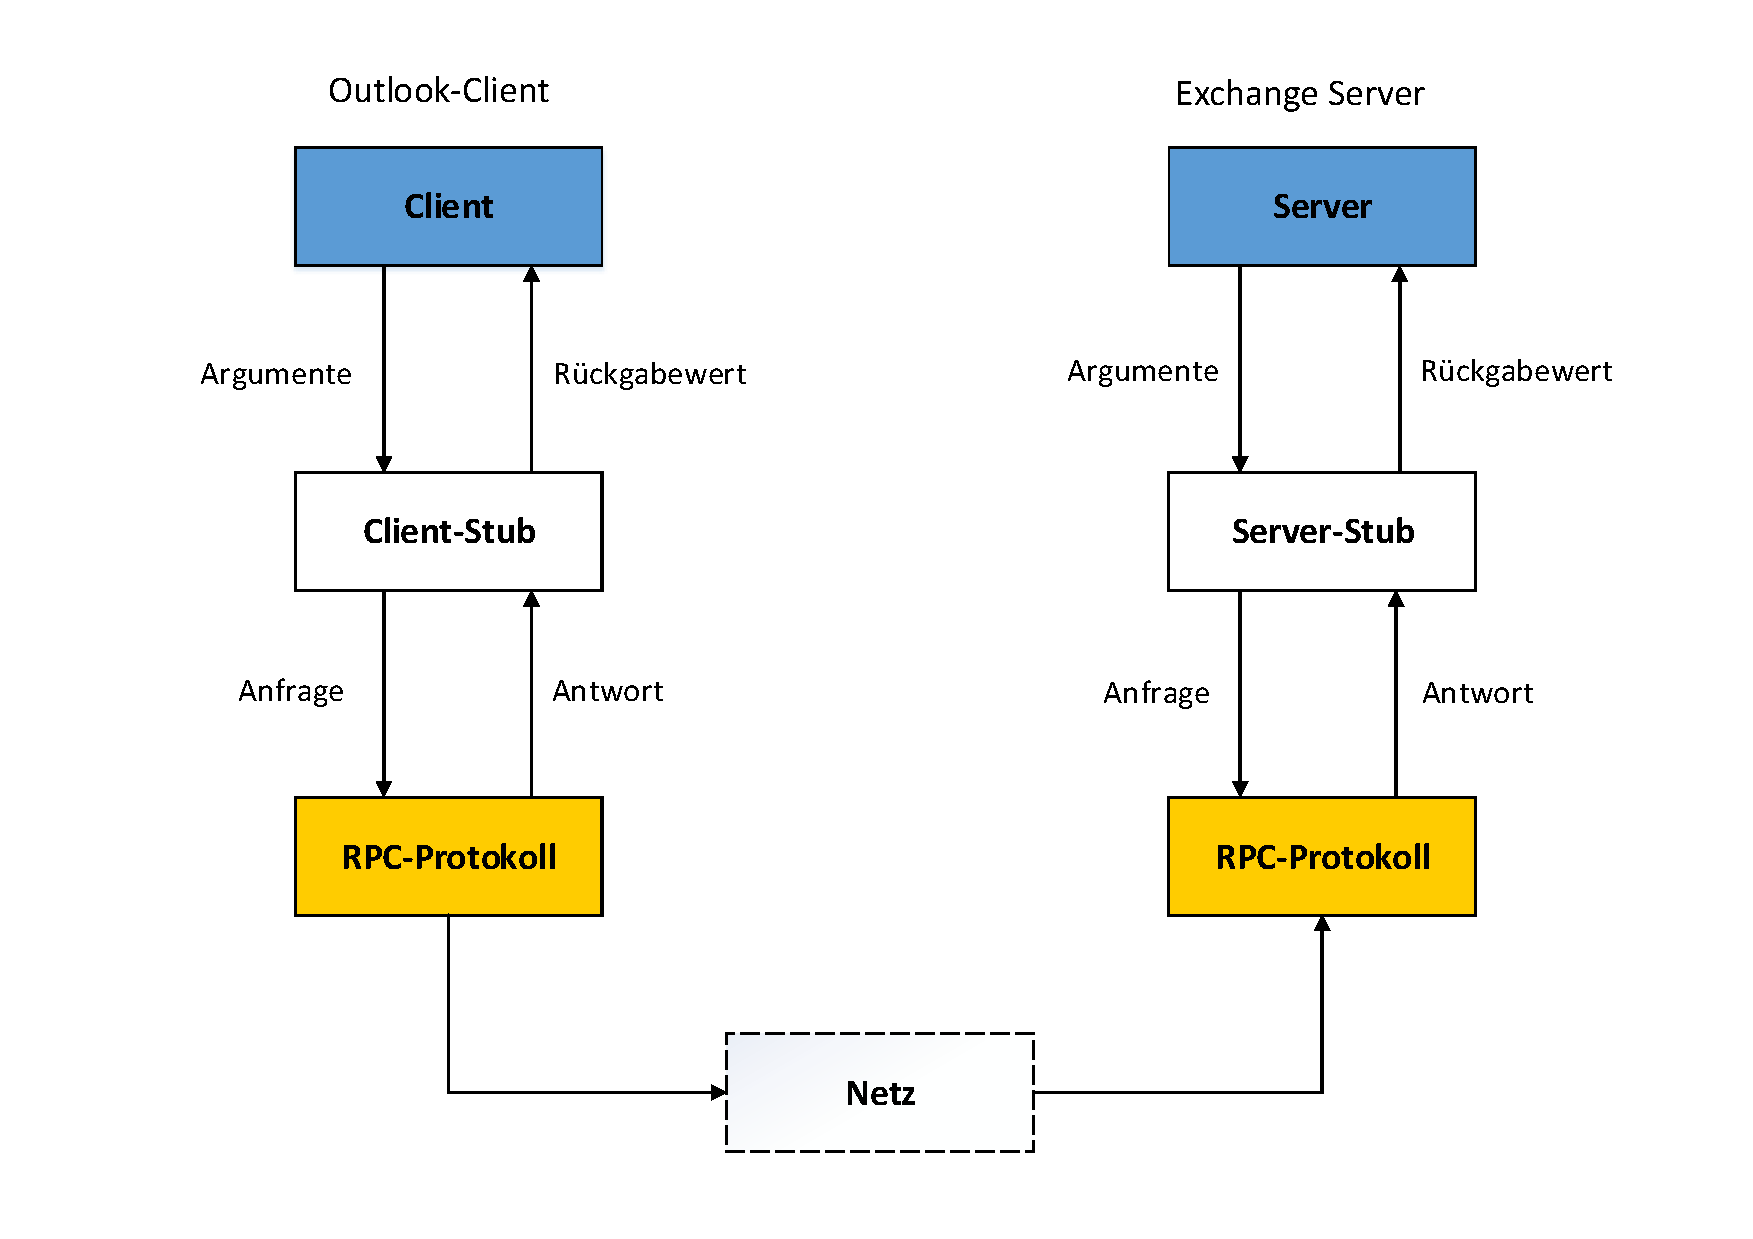
\includegraphics[width=0.59\textwidth]{Abbildungen/RPC_TCP}
	\caption[Aufbau einer klassischen RPC Verbindung]{Aufabu einer klassischen RPC Verbindung,    in Anlehnung an:\\https://technet.microsoft.com/de-de/library/e8feb37e-f3a9-4f26-bed0-6583d8a110ed}
	\label{fig:RPC_TCP}
\end{figure}

\noindent 
Der Client ruft eine Prozedur mit spezifischen Argumenten (Eingabeparameter) auf. Der Client-Stub aktiviert eine gleichnamige Prozedur und wandelt die Argumente in ein plattformunabhängiges Datenformat um. Die Daten werden dann über das Netz mithilfe des TCP/IP-Protokolls an den Server geschickt. Dort erhält der Server-Stub die Anfrage und wandelt die Argumente in das lokale Format des Servers um. Nun ruft der Server die gewünschte Prozedur mit den Eingabeparametern auf und der Rückgabewert kehrt in den Server-Stub zurück. Nach einer erneuten plattformunabhängigen Umwandlung der Datenformate, wird die Antwort an den Client-Stub geschickt. Im letzten Schritt erhält der Client die in das lokale Format umgewandelte Antwort (Rückgabewerte) auf seine Anfrage.\footnote{Vgl. \citeauthor{Schneider} (\citeyear{Schneider}), S.406 f.}\newline
Ab Exchange 20013 wird der Datenaustausch zwischen dem Outlook-Client und dem Exchanger Server standardmäßig über RPC/HTTP (auch Oulook Anywhere genannt) geregelt. Wie der Name schon vermuten lässt, läuft die gesamte Kommunikation bei dieser Variante über HTTP bzw. HTTPS. Somit kann über das Internet auf den Exchange Server zugegriffen werden. Outlook Anywhere ist besonders für Mitarbeiter geeignet, die von zu Hause auf ihr Exchange-Postfach zugreifen möchten, da sie sich nicht im Unternehmensnetzwerk befinden müssen.\footnote{Vgl. \citeauthor{Joos} (\citeyear{Joos}), S. 33, S. 254.}

\begin{figure}[h!]
\centering
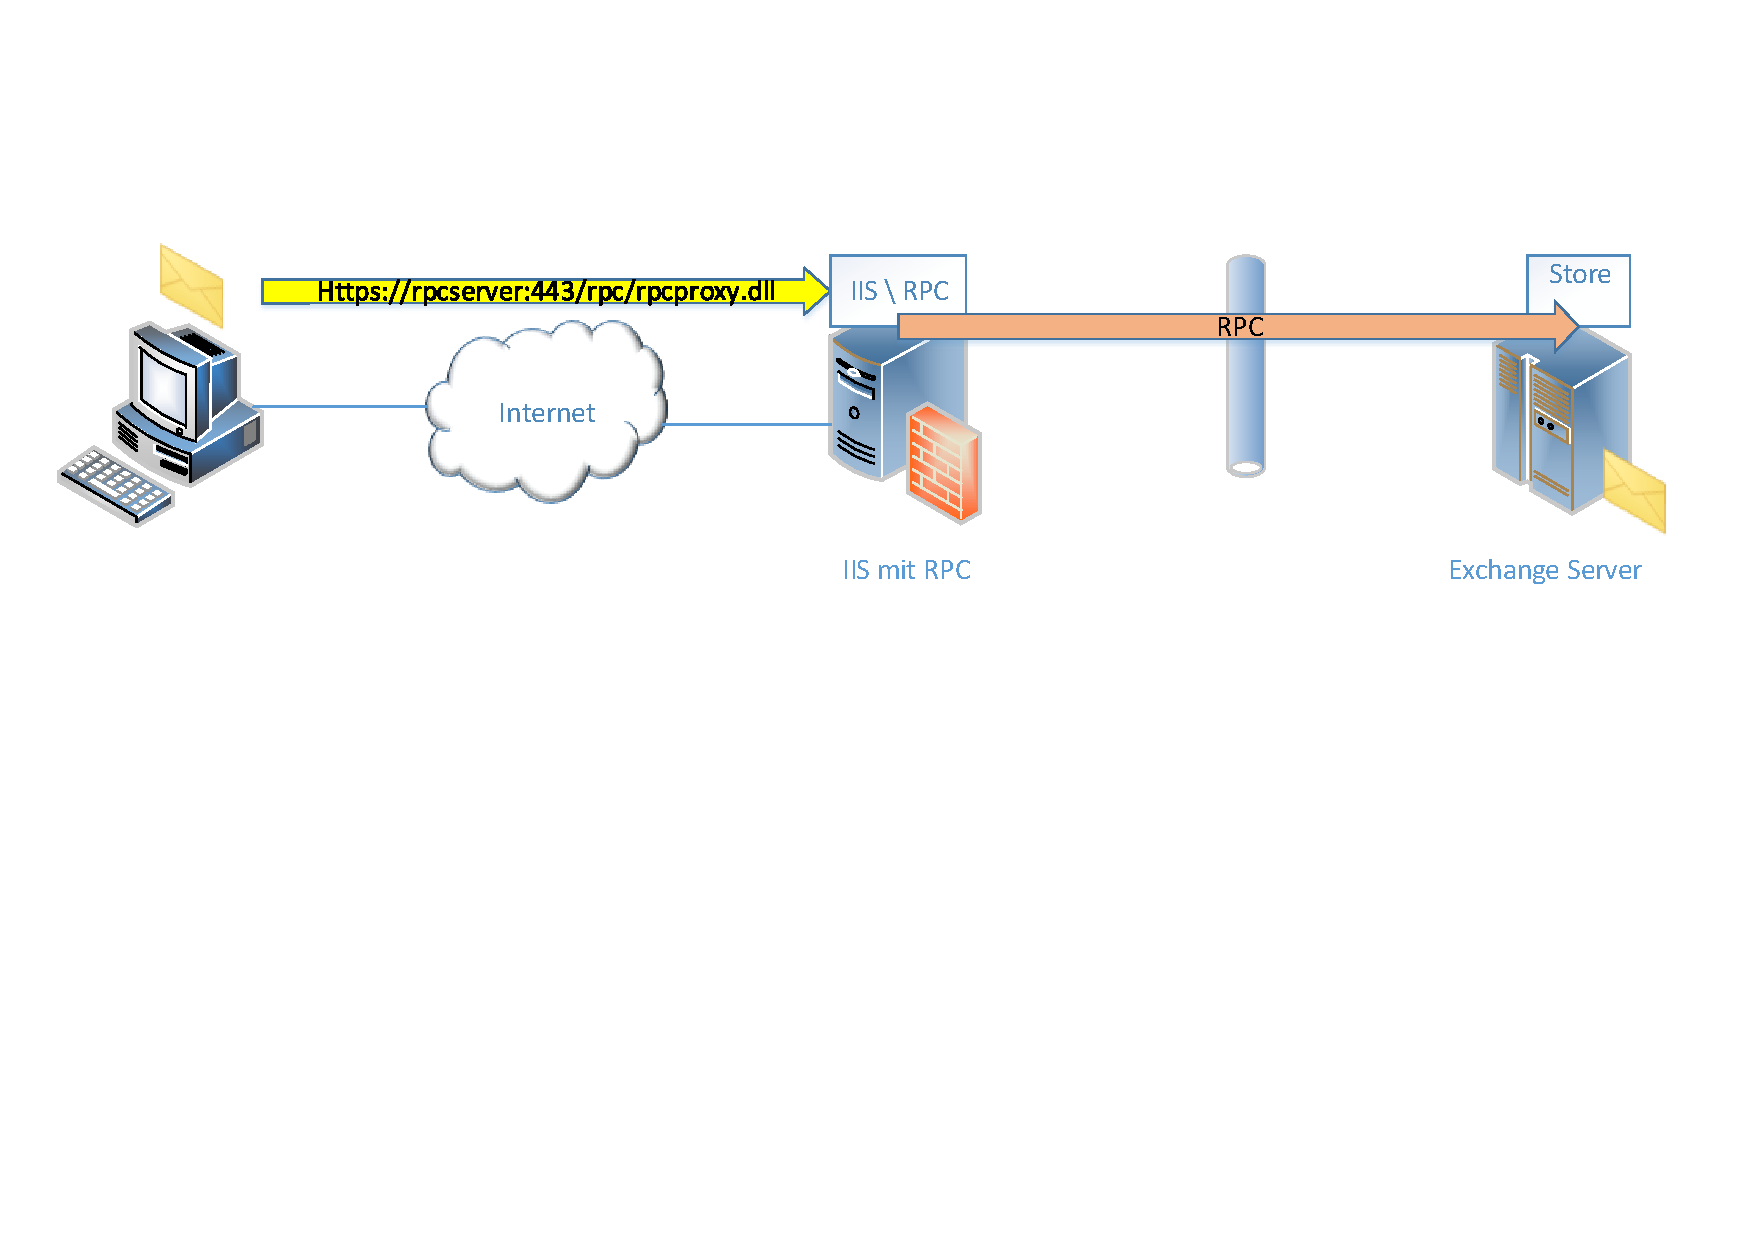
\includegraphics[width=0.65\textwidth]{Abbildungen/RPC_HTTP}
	\caption[RPC over HTTP Prinzip]{RPC over HTTP Prinzip,  in Anlehnung an:http://
	www.msxfaq.de/clients/oagrundlagen.htm}
	\label{fig:RPC_HTTP}
\end{figure}

\noindent
In der Abbildung \ref{fig:RPC_HTTP} sieht man deutlich, dass der Outlook-Client über HTTPS mit dem IIS kommuniziert, auf dem ein virtuelles RPC-Verzeichnis existiert. Der IIS ist eine Microsoft-Webserverplattform, die Webanwendungen und Dienste bereitstellen und verwalten kann.\footnote{Vgl. \citeauthor{Volodarsky} \citeyear{Volodarsky}, S.3.} Der IIS wiederum, baut über einen RPC-Proxy eine Verbindung mit dem Exchange Server auf. Wichtig ist hierbei, dass die Kommunikation des Clients sich auf HTTP oder HTTPS beschränkt.\footnote{Website:\cite{MSXoutlook}}


\subsection{Exchange Web Services}
\noindent
Die Grundlagen von Mircosoft Exchange Server sind geklärt. Doch wie können nun Programmierer über Quellcode auf den Exchange Server zugreifen. Hierfür hat Mircosoft im Laufe der Jahre eine Reihe von Programmierschnittstellen bereitgestellt. Eine Schnittstellen zur Anwendungsprogrammierung wird als API (englisch application programming interface) bezeichnet. Es ist nicht nötig, alle Programmierschnittstellen zu erläutern, da eine Vielzahl der APIs keine Verwendung mehr finden oder nicht mehr unterstützt werden. Zu Informationszwecken befindet sich jedoch im Anhang auf Seite~\pageref{API_1} eine Übersicht einiger Programmierschnittstellen ab dem Jahr 1992. Ab Exchange 2007 setzt Microsoft immer mehr auf den Exchange Web Services (kurz EWS) als Programmierschnittstelle und baut diese seitdem weiter aus.\footnote{Website:\cite{MSXews}}
Redmond schreibt im Handbuch Exchange 2010: 
\enquote{Abgesehen von Windows PowerShell liegt der Schwerpunkt für die meisten Entwickler jetzt auf der API EWS (Exchange-Webdienste), die in Exchange Server 2007 eingeführt wurde.}\footnote{\citeauthor{Redmond} \citeyear{Redmond}, S.634.}
Er macht deutlich, dass EWS die erste Anlaufstelle für Entwickler ist. Eine weitere Programmierschnittstelle namens REST API erschien 2015 mit Office 365. Der REST API wird aber keine weitere Beachtung geschenkt, da sie lediglich in der Office 365-Umgebung Anwendung findet.\footnote{Website:\cite{MicrosoftAPI}}


\subsubsection{Funktionsweise}
\noindent
Standardmäßig bildet das Simple Object Access Protocol (kurz SOAP) eine Grundlage für Web-Services. Schneider beschreibt SOAP als \enquote{ein RPC-Mechanismus, bei dem die übertragenen Daten im XML-Format codiert werden.}\footnote{\citeauthor{Schneider} \citeyear{Schneider}, S.407.}
Schill und Springer schreiben genauer: \enquote{Das objektorientierte Kommunikationsprotokoll SOAP ermöglicht die Kommunikation zwischen heterogenen Diensten unter interner Nutzung
des Hypertext Transfer Protocol (HTTP) und mit Kodierung der Parameter in der eXtensible Markup Language (XML).}\footnote{\citeauthor{Schill} \citeyear{Schill}, S.69.}
Auch die Exchange Web Services funktionieren nach diesem Prinzip.\footnote{Website:\cite{MicrosoftSDK}}
 
\noindent
Mit Exchange 2007 wurde erstmals der Exchange Web Services  bereitgestellt und löste nach und nach andere APIs ab. Die nachfolgende Abbildung zeigt, wie sich EWS seit 2007 entwickelt hat.

\begin{figure}[h!]
\centering
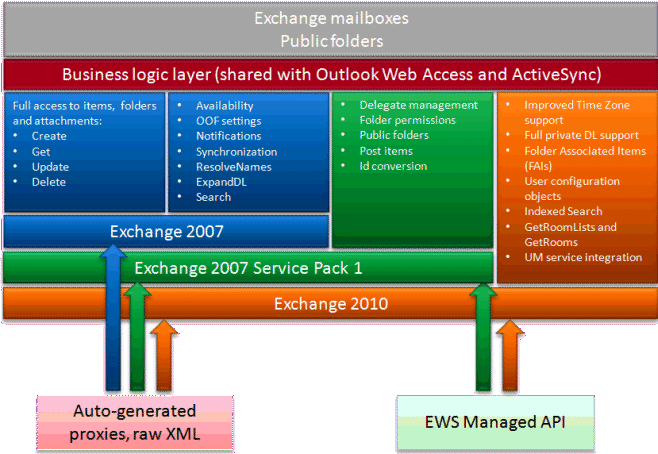
\includegraphics[width=0.65\textwidth]{Abbildungen/EWS_Funktionsumfang.png}
	\caption[EWS Funktionsumfang]{EWS Funktionsumfang, Quelle: http://www.msxfaq.de/code/
	ews.htm}
	\label{fig:EWS_Funktionsumfang}
\end{figure}

\noindent
EWS bietet einen großen Funktionsumfang und ist somit eine hervorragende Möglichkeit auf die Daten des Exchange Servers zuzugreifen. Aus diesem Grund haben sich die Entwickler der KMS Computer GmbH für diese Programmierschnittstelle entschieden.

\subsubsection{Derzeitige Verwendung in GEBman 10}
\noindent
Um bei der Implementierung den Exchange Web Service nutzen zu können, musste die Microsoft Exchange Web Services Managed API 2.2. dem Projekt als .NET-Assembly hinzugefügt werden. Wie bereits im Punkt 4 erwähnt, kann im Adminbereich von GEBman10 kann in der der Rubrik GroupWare die Konfiguration des Exchange Servers durchgeführt werden. Wichtig ist hierbei zunächst, welche Version vom Exchnage Server verlangt wird, da das entscheidend für die Microsoft Web Services Managed API ist. GEBman10 unterstützt folgende Exchange Server-Versionen:

\begin{itemize}[topsep=-0.5\parskip]
\item Exchange 2007 inkl. SP1
\item  Exchange 2010 inkl. SP1
\item  Exchange 2013 
\end{itemize}

\noindent
Nachdem die Version bestimmt und die Benutzerdaten eingetragen wurden, kann direkt im Code mittels der API direkt auf den Exchange Server zugegriffen werden. Derzeit ist das Versenden von E-Mails über den Code implementiert, sodass eine Grundlage für die Erweiterung bereits vorhanden ist. Auch das Auswerten von E-Mails ist über diese API möglich und eine Schnittstelle muss nicht mehr implementiert werden. Diese vorhandenen Funktionalitäten werden als Grundlage für die folgenden Konzipierung und anschließende Implementierung genutzt. 

\newpage

%-------------------------------------------------------------------------------------------------------
%					6	Konzipierung
%-------------------------------------------------------------------------------------------------------

% !TEX root = Bachelorarbeit_Paul_Zilewitsch.tex
\section{Konzipierung}
\subsection{Analyse aus Kapitel 1 und Kapitel 2 (UML-Diagramme etc.)}
\subsection{Zielsetzung}
\subsection{Sicherheitsaspekte}
\noindent
Immer wieder vernachlässigen Entwickler die Sicherheit ihrer Implementierungen. Das liegt meistens an mangelnder Zeit, da Releases einen festen Zeitplan verfolgen, den es einzuhalten gilt. Es kann aber auch sein, dass die Implementierung nicht aus dem Blickwinkel der Sicherheit betrachtet wird. "Hauptsache es funktioniert erst einmal", wird dann häufig als Argument genutzt. Natürlich hat das wenig mit Sicherheit zu tun. Dabei können es Entwickler mit wenig Aufwand, Angreifern deutlich schwerer machen. Deswegen werden im nachfolgendem zwei Sicherheitsprobleme für die Umsetzung des Konzepts in GEBman 10 besprochen. Die Abbildung XX zeigt zwei kritische Bereiche, die genauer erläutert werden müssen.

\begin{figure}[h!]
\centering
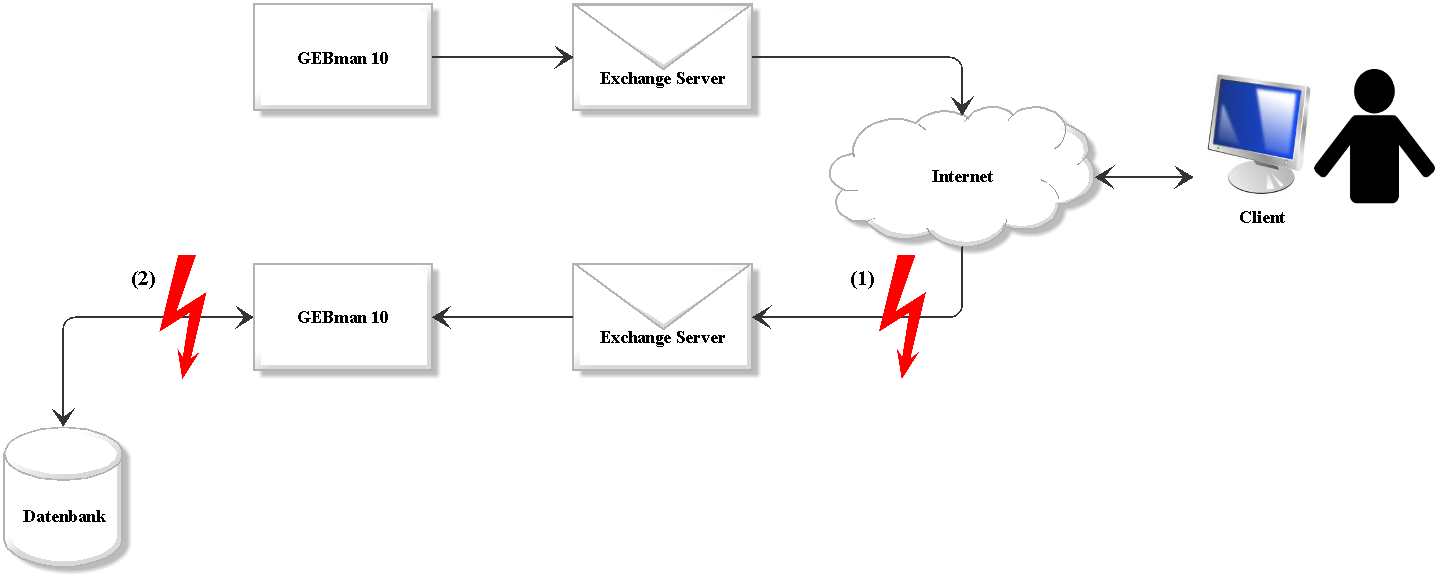
\includegraphics[width=0.85\textwidth]{Abbildungen/Sicherheitsprobleme.png}
	\caption[Sicherheitsprobleme]{Sicherheitsprobleme, Quelle:eigene Darstellung}
	\label{fig:Sicherheitsprobleme}
\end{figure}

\noindent
Der rechte rote Blitz - gekennzeichnet mit der (1) - symbolisiert das erste Problem.

\noindent
Beim zweiten roten Blitz der Abbildung XX - gekennzeichnet mit der (2) - wird uns die Arbeit nicht wie beim ersten kritischen Bereich abgenommen. GEBman 10 synchronisiert in regelmäßigen Abständen die Nachrichten vom hinterlegten Exchange Server. Entsprechend ihrer ID werden die Nachrichten in die Datenbank von GEBman 10 gespeichert. Nun könnte ein Angreifer beispielsweise versuchen, in den Mail-Body versteckte SQL -Anweisungen oder JavaScript-Code einzuschleusen. Werden die SQL-Anweisungen in die Datenbank geschrieben, ohne sie vorher zu validieren, könnte der Angreifer Informationen über Daten in der Datenbank erlangen. Im schlimmsten Fall könnte er sie zerstören. Diese Angriffstmethode nennt sich SQL-Injection und zielt darauf ab, die normalen SQL-Statements mittels Sonderzeichen zu manipulieren. Selbst einfache Zeichen wie "--" können bewirken, dass alles, was hinter den beiden Bindestrichen steht, ignoriert wird. In T-SQL sind die beiden Bindestriche das Zeichen für einen Kommentar.
\noindent
Bei JavaScript-Code haben wir ein ähnliches Problem mit bestimmten Zeichen. Wird zum Beispiel die einfache Zeichenfolge "<script>alert('hallo')<script>" in die Datenbank geschrieben, passiert ersst einmal gar nichts. Die SQL-Statements werden hierdruch nicht manipuliert. Doch wird diese Zeichenfolge beispielsweise als Antwort auf eine Meldung geladen, erkennt der Browser möglicherweise JavaScript-Code anstatt einfachen Text. Das hat in unserem Beispiel zur Folge, dass der Browser eine kleine Nachricht meldet (siehe Abbildung).
Auch hier muss vor dem Einfügen der Zeichenfolge, eine Validierung vollzogen werden. Welche Zeichen genau gefiltert werden müssen, wird im Punkt 5 Umsetzung erläutert. Man sollte sich jedoch nicht darauf verlassen, dass die Schutzmechanismen des Microsoft Exchange Servers alle Zeichen und Zeichenfolgen als Bedrohung erkennen. Zeichen wie "--" oder ">" können durchaus im normalen Schriftverkehr gebräuchlich sein.
\noindent
Es gibt für Angreifer noch mehr Angriffsmöglichkeiten beispielsweise zwischen Client und Internet/Server über Man-in-the-Middle etc.. Darauf soll aber in dieser Arbeit nicht weiter eingegangen werden, da das ein sehr umfangreiches Thema ist und eine eigenständige Bachelorarbeit bilden könnte. Eins sollte jedem klar sein: Hat ein Cracker genügend Zeit und Ressourcen, ist ein System, das über das Internet kommuniziert, äußert schwer vollkommen zu sichern. 
\noindent
Durch die Analyse aus Punkt 2 und Punkt 3 konnte ein genaues Ziel gesetzt werden. Die Funktionsweise der Exchange Web Services sind geklärt und auch Sicherheitsaspekte wurden berücksichtigt. Die Konzipierung ist somit abgeschlossen und er Implementierung steht nichts mehr im Wege.

\newpage

%-------------------------------------------------------------------------------------------------------
%					7	Ummsetzung
%-------------------------------------------------------------------------------------------------------

% !TEX root = Bachelorarbeit_Paul_Zilewitsch.tex
\section{Umsetzung}

\subsection{Erweiterung des bestehenden Service Desk Moduls}
\noindent
Grundlage für die Erweiterung ist die bereits erwähnte Microsoft Exchange Web Services Managed API 2.2, die kostenlos zum Download von Microsoft angeboten wird. Voraussetzung für diese API ist ein Betriebssystem von Windows (mindestens Windows 7) und das .NET Framwork 3.5 oder höher.\footnote{Website:\cite{DownloadAPI}}\newline 
Da diese API bereits in GEBman10 für das Versenden von E-Mails integriert wurde, konnte direkt ohne zusätzlichen Aufwand auf die Funktionalitäten zugegriffen werden. Wichtig war lediglich das Einfügen des Assemblerverweises in die entsprechenden Projektmappenordner. Um nicht den vollständigen Namespace jeder Klasse ausschreiben zu müssen, wurde außerdem die using-Direktive in den Klassen MailsToObjectsFactory und TicketHandler hinzugefügt.

\begin{figure}[h!]
\centering
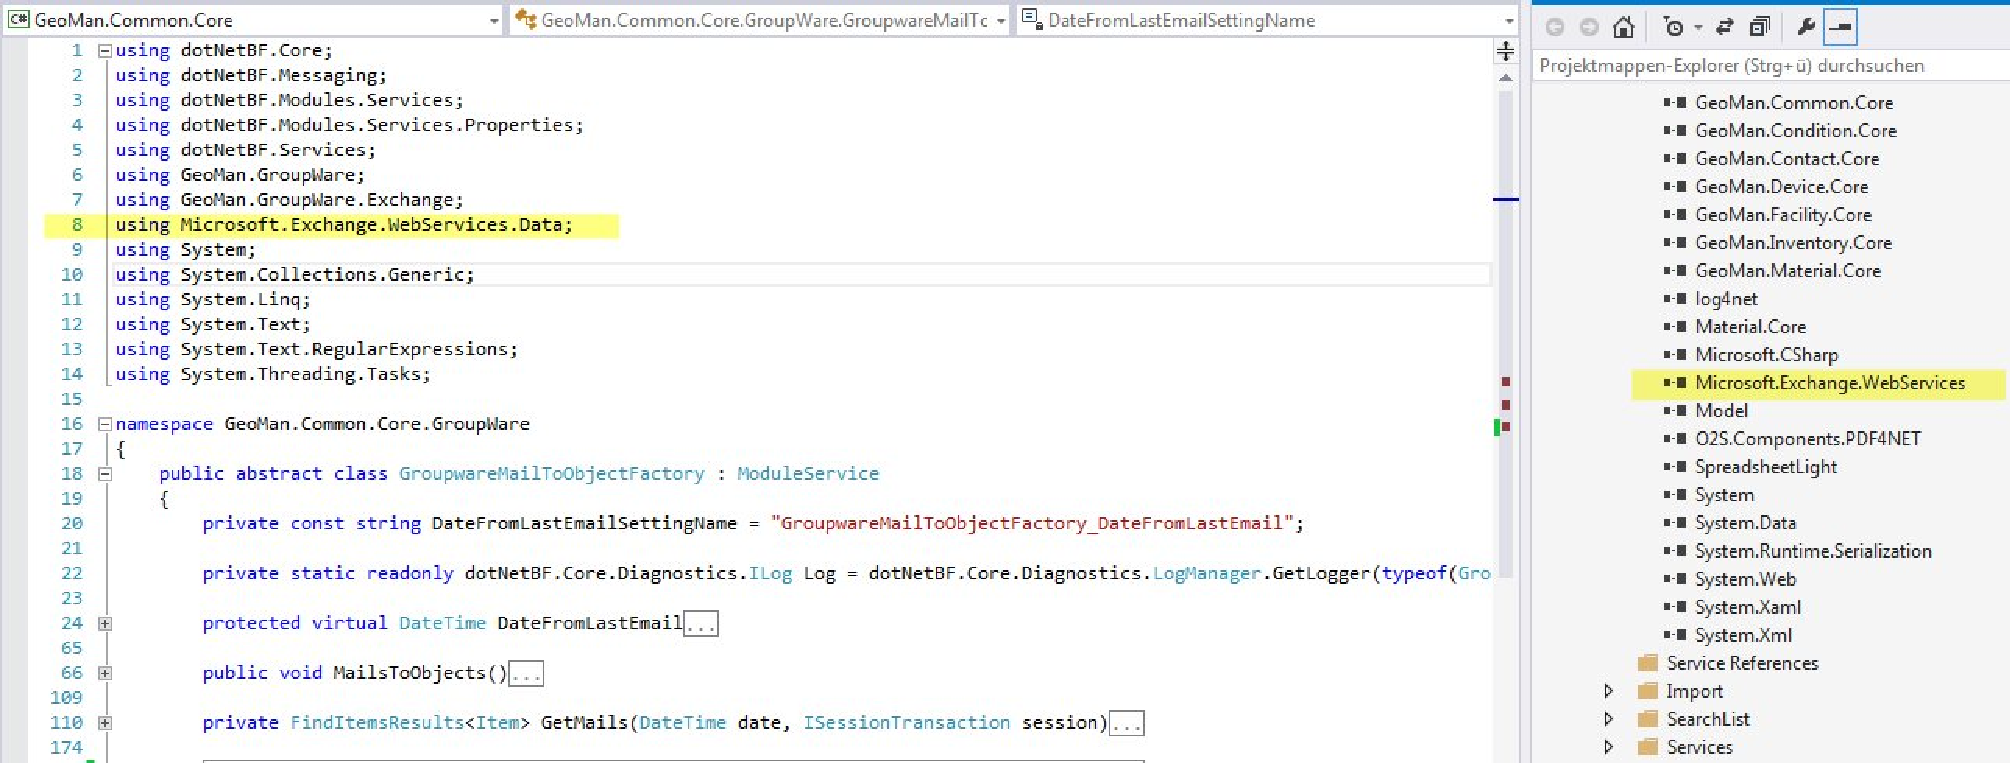
\includegraphics[width=0.75\textwidth]{Abbildungen/Screenshot_Verweise.pdf}
	\caption[Verweise]{Entwurfsmuster Fabrikmethode, Quelle: eigene Darstellung}
	\label{fig:Verweise}
\end{figure}

\noindent
Bei der Implementierung wurde sich stark an das Fabrikmethoden-Entwurfsmuster gehalten. Bevor hierauf näher eingegangen wird, sollte das Entwurfsmuster näher erläutert werden.\\
\noindent
Die Fabrikmethode (Factory Method) ist ein Erzeugungsmuster, bei dem die Objekterstellung von der Objektverarbeitung getrennt wird. Hierbei wird die Unterklasse durch eine abstrakte Methode der Oberklasse erzeugt.\footnote{Vgl. \citeauthor{PatternsKompakt} \citeyear{PatternsKompakt}, S.34ff.} Dieses Entwurfsmuster wurde auch bei der Implementierung in GEBman10 verwendet. 

\begin{figure}[h!]
\centering
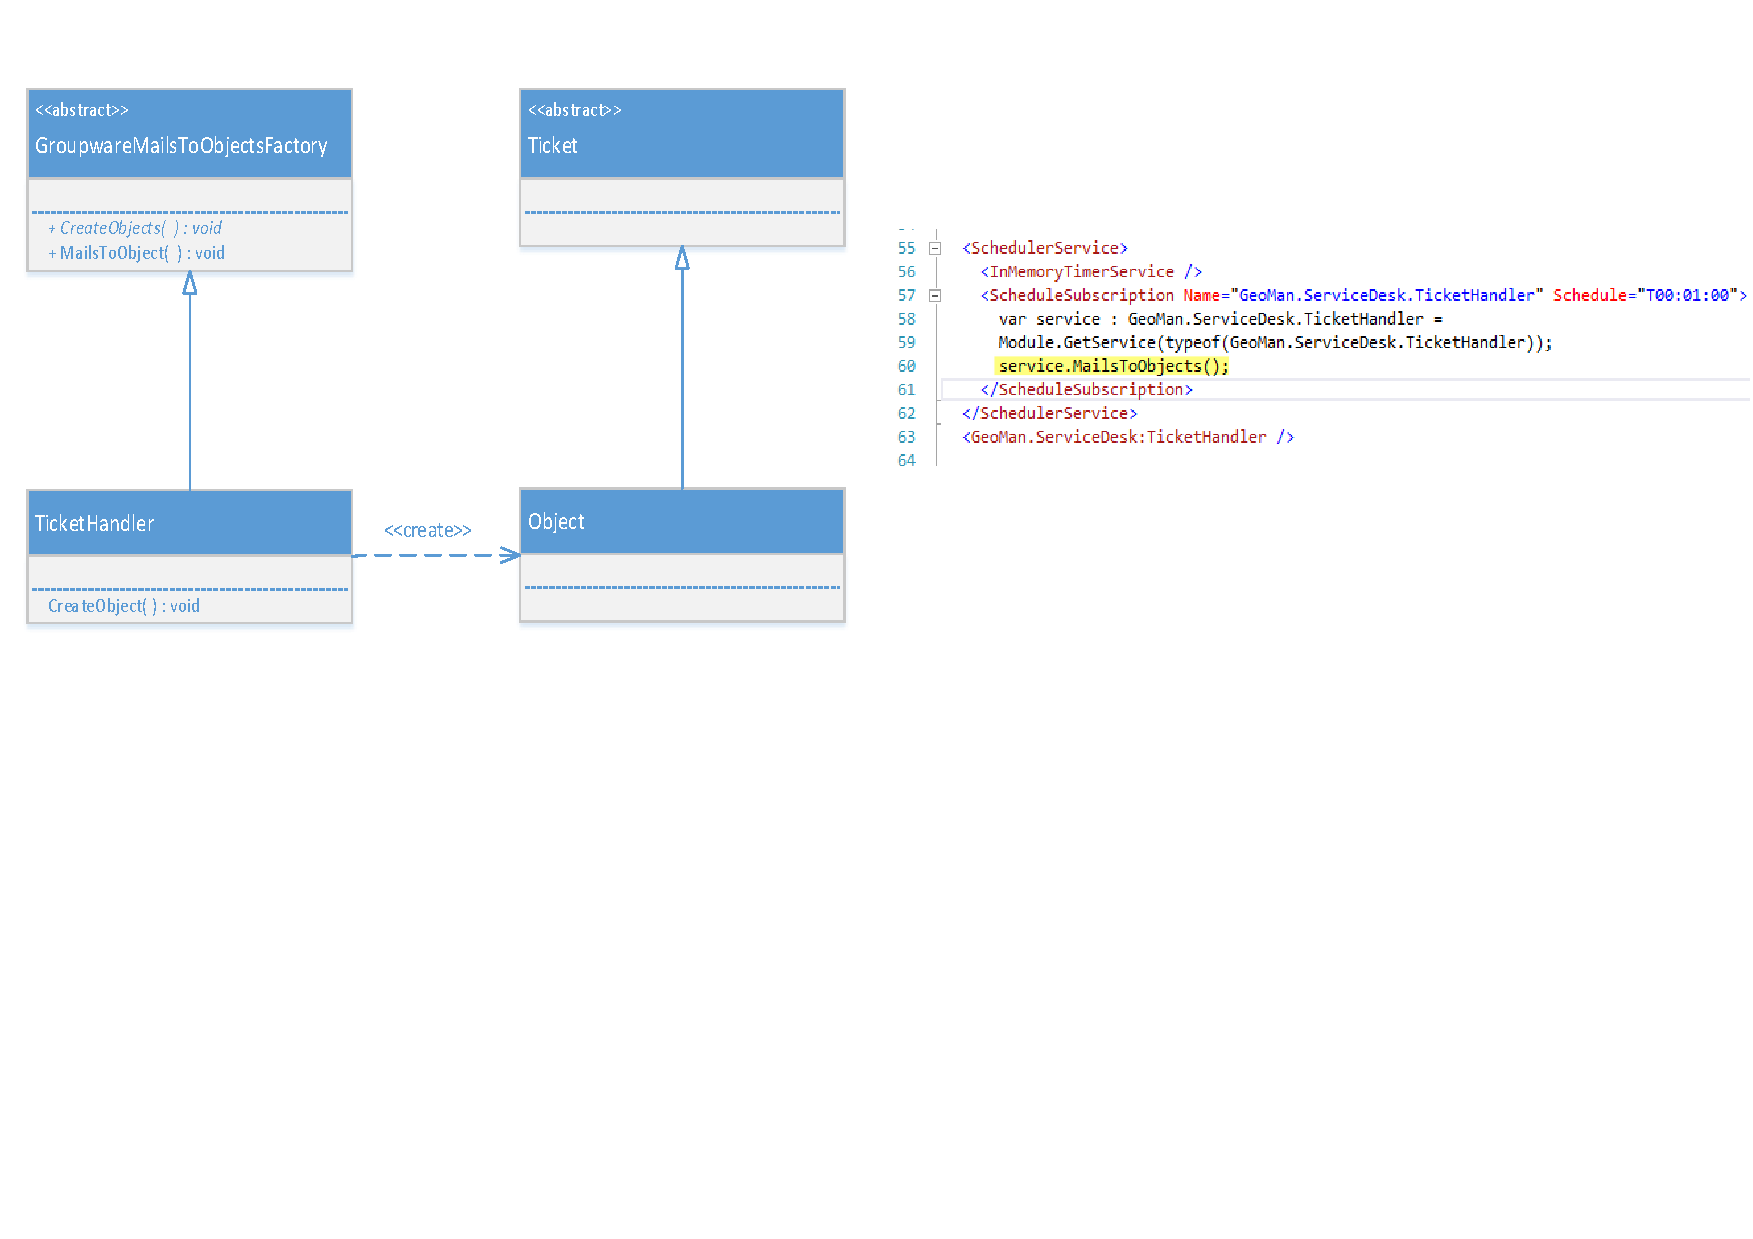
\includegraphics[width=0.9\textwidth]{Abbildungen/Entwurfsmuster.pdf}
	\caption[Entwurfsmuster Fabrikmethode]{Entwurfsmuster Fabrikmethode, Quelle: in Anlehnung an Eilebrecht, Starke (2013) S.35}
	\label{fig:Entwurfsmuster}
\end{figure}

\noindent
Bei jedem Intervall wird über den SchedulerService (Abbildung~\ref{fig:Entwurfsmuster} links) der Module Service TicketHandler instanziiert und die Methode MailsToObjects( ) der abstrakten Oberklasse aufgerufen. Die Fabrikmethode (rechts) macht deutlich, dass die abstrakte Klasse GroupwareMailToObjectFactory der Erzeuger und Ticket Handler der konkrete Erzeuger ist. Der konkrete Erzeuger wiederum erstellt dann ein Object über die abstrakte Methode CreateObject( ). Das Object ist in diesem Falle ein Ticket (Meldung). Vorteil dieses Entwurfsmusters ist die klare Kapselung des Erzeugers. Somit kann die Klasse GroupwareMailToObjectFactory auch für andere Module eingesetzt werden, die ebenfalls neue Objekte aus E-Mails erzeugen sollen. Eilebrecht und Starke sehen die Anwendung der Fabrikmethode als sinnvoll, wenn \enquote{eine Klasse die von ihr zu erzeugenden Objekte nicht im Voraus kennt}.\footnote{Vgl. \citeauthor{PatternsKompakt} \citeyear{PatternsKompakt}, S.34ff.} Genau dieser Anwendungsfall trifft hier zu und ist deshalb auch gerechtfertigt.\\






\subsection{Erläuterung einzelner Methoden}
\noindent
Die Methode GetMails( ) in der Klasse GroupwareMailsToObjectFactory ist die entscheidene Methode der Erweiterung bei dem Abrufen der E-Mails eines Exchange Servers. Hier werden nicht nur alle Mails abgerufen, sondern auch verschiedene Attribute der einer E-Mails geladen. Im Anhang auf Seite XX ist ein Ausschnitt des Quellcodes abgebildet. Zu sehen ist, wie...\\

\noindent
Das erstellen einer Meldung (Objektes) erfolgt in der Methode CreateObject( ). Diese Methode ist in der GroupwareMailsToObjectFatory als abstrakte Methode definiert, wird der Klasse TicketHandler vererbt und hier auch explizit aufgerufen. Wichtig bei diese Methode ist die Übergabe einer Session. In GEBman10 benötigt jede Datenbankbearbeitung eine neue SessionTransaction.\footnote{Vgl. \citeauthor{Fowler} \citeyear{Fowler}, S.103ff.} 
Mithilfe der Session lässt sich somit auf die Create-Methode der Ticket Klasse zugreifen. Anschließend werden die Eigenschaften des E-Mail-items den zuvor angedeuteten nötigen Eigenschaften eines Tickets zugewiesen. Nach diesem Prozess wird die Session committed, um die neu erstellte Meldung in der Datenbank zu speichern. Erst jetzt erhält die Meldung eine eindeutige ID. Diese ID kann dazu genutzt werden, um im nächsten Schritt einen möglichen Anhang der E-Mail zu speichern. Das übernimmt die Methode SaveAttachment( ). In dieser Methode wird zunächst ein Dokument mit dem selben Inhalt des Anhangs der E-Mail erstellt. Dann wird dieses Dokument dem entsprechenden Ticket mit Hilfe der übergebenen ID zugeordnet. Wurden diese Anweisungen erfolgreich durchgeführt, wird eine Bestätigungsmail mit der Methode SendConfirmationMail( ) gesendet.\\

\noindent
Bei jedem Versuch die Datenbank zu verändern, kann es zu Fehlern kommen, die dem Benutzer auch mitgeteilt werden müssen. Der Benutzer muss schließlich darüber informiert werden, wenn eine Meldung nicht korrekt angelegt wurde. Aus diesem Grund wurden try-catch-Anweisungen bei jedem Datenbankzugriff verwendet. Durch diese try-catch-Anweisungen werden Ausnahmen beim Ausführen des Codes abgefangen. Dadurch ist es möglich, eine Ausnahmebehandlung zu vollziehen.\footnote{Website:\cite{TryCatch}}


\subsection{Testfälle}
\noindent
In den letzten Jahren hat sich das Testen von Software zunehmende etabliert und ist ein fester Bestandteil von Softwareprojekten für die Qualitätssicherung..\footnote{Vgl.\citeauthor{Vivenzio} \citeyear{Vivenzio}, S.1f.} Deshalb werden auch bei der Erweiterung des Service Desk Moduls einige Testfälle die wichtigsten Funktionalitäten überprüfen. Hierfür muss zunächst ein Testablauf erarbeitet und ein die zu erwartenden Werte des Testresultats festgehalten werden.\newline
Bei den Testfällen in GEBman 10 wird im ersten Schritt der Webserver gestartet. Dadurch wird auch der implementierte ModulService TicketHandler initialisiert. Nun werden alle Modultests ausgeführt. Für den Test des ModulService wird ein Exchange Server benötigt. Dieser wird mittels einer Methode in der TestHelper-Klasse angelegt. An diesen Exchange Service wird eine E-Mail gesendet und anschließend der ModulSerive aufgerufen. Theoretisch könnte der Modultest auch bis zum nächsten Intervall des Modul Service warten, bis dieser die neuesten Mails vom Exchange Server abfragt. Doch ein Modultest sollte so wenig Zeit wie möglich beanspruchen. Aus diesem Grund wird die Methode MailsToObjects vom ModulService manuell aufgerufen. Eine neue Meldung wird aus der zuvor gesendeten E-Mail erstellt. Erst jetzt beginnt der eigentliche Test. Es wird eine Datenbankabfrage erstellt, die nach der Meldung sucht, die der ModulService angelegt haben müsste. Sollte die Abfrage erfolglos sein, wird der Modultest mit einem Fehler beendet. Sollte die Meldung gefunden werden, wird im nächsten Schritt geprüft, ob der Anhang der E-Mail als Dokument der Meldung angelegt wurde. Wurde kein Dokument gefunden, dass der zuvor erstellten Meldung zugeordnet ist, schlägt der Modultest fehl und eine entsprechende Meldung wird ausgegeben.\newline
Die Testfälle können noch weiter ausgebaut werden, in dem weitere Methoden implementiert werden, die eine erfolgreiche Antworterstellung oder das Versenden von Bestätigungsmails prüfen. Abschließend ist festzuhalten, dass niemals alle möglichen Szenarien in Testfällen berücksichtigt werden können, aber auch gar nicht müssen. Es geht lediglich darum, die Szenarien zu testen, die am häufigsten in der Praxis auftreten.\footnote{Vgl.\citeauthor{Witte} \citeyear{Witte}, S.11f.}


\subsection{Fehlschläge/Erfahrungen}
\noindent
Bei der Implementierung in GEBman10 gab es zwei nicht vorhersehbare Probleme bei der Implementierung. Beide haben ihren Ursprung in der Managed API von Microsoft. In der Methode GetMails( ) werden alle Mails aus dem Posteingang des Exchange Servers abgefragt. Hierfür stellt die API eine Methode namens FindItems( ) zur Verfügung, die eine Collection aller Items liefert. Nun muss aber für diese Collection eine ItemView übergeben werden, die einen bestimmten Integerzahlenwert als festdefinierte Größe benötigt. Es ist also in der Theorie durchaus möglich, dass sich mehr Mails im Posteingang des Exchange Server befinden, als die Menge an Elementen der ItemView. Das hat zur Folge, dass alle Mails außerhalb der ItemView nicht in die Collection von der Methode FindItems( ) enthalten sind und auch nicht ausgewertet werden können. Um dieses Problem kurzer Hand zu beseitigen, wurde die ItemView Größe auf den maximalen Zahlenwert des Integerwertebereiches gesetzt. Dieses Wert zu überschreiten ist in der Praxis so gut wie unmöglich, der sich in einem 10-stelligen Bereich bewegt.\\
%Es gäbe noch einen anderen WorkAround für dieses Problem, allerdings wäre diese Lösung mit mehr Aufwand verbunden. 
%https://msdn.microsoft.com/en-us/library/office/dd633698(v=exchg.80).aspx

\noindent
Das zweite Problem bestand bei der Abfrage der neusten Mails vom Exchange Server, ebenfalls in der GetMails( )-Methode beschrieben. Bei jedem Abfrage Intervall wird der Zeitpunkt der zuletzt eingetroffenen Mail gespeichert. Beim nächsten Intervalldurchlauf werden dann nur alle Mails abgefragt, die ein aktuelles Datum besitzen. Hierfür bietet die Managed API einen SearchFilter an, der die Mails nach definierten Eigenschaften suchen kann. In diesem Fall ist war die Filter-Methode IsGreatherThan( ) optimal für dieses Vorhaben. Theoretisch hätten alle Mails abgefragt werden müssen, die ein \enquote{größeres} und damit aktuelleres Datum als die zuletzt eingetroffene Mail vom vorherigen Intervalldurchlauf hatten. Tatsächlich hat sich beim Debuggen gezeigt, dass der Filter zusätzlich ebenfalls die Mails liefert, die das gleiche Datum besitzen. Dadurch würde eine Mail in jedem Intervall zweimal gefiltert werden, was eine womöglich redundante Objekterzeugung zur Folge hätte. Wodurch dieses Problem entstand bleibt unklar. Umgangen wurde es, indem dem Datum der zuletzt eingetroffenen Mail nur eine Sekunde hinzugefügt wurde. Nach dieser minimalen Veränderung wurden die Mails korrekt gefiltert.


\subsection{Erweiterungsmöglichkeiten der E-Mail Integration}
\noindent
Die E-Mail Integration könnte dahingehend erweitert werden, dass der Benutzer mit einer E-Mail mehr Möglichkeiten zum Verändern vorhandener Meldungen hat. Sollte ein Benutzer beispielsweise den Status einer Meldung auf \enquote{Technisch fertig setzen} setzen wollen, könnt er das über eine E-Mail bewerkstelligen, ohne dabei in GEBman 10 eingeloggt sein zu müssen. Denkbar wäre es, in den Betreff der E-Mail einen Parameter wie \enquote{\#fertig} einzusetzen. Beim Auslesen der E-Mails durch den ModulService könnte das erkannt werden und dem Absender der E-Mail könnte ein Link geschickt werden. Mit diesem Link könnte der Benutzer dann zu einem temporären Webfrontend gelangen, auf dem dann die Fertigstellung der Meldung noch einmal bestätigt.\\\\
\noindent
In GEBman 10 können mehrere Benutzer mit ihren E-Mail Adressen hinterlegt werden. Der Modul Service könnte abgleichen, ob ein Absender einer E-Mail im Exchange Postfach eine identische E-Mail Adresse wie ein registrierter Benutzer in GEBman 10 hat. Ist die E-Mail Adressen eines hinterlegten Benutzer identisch mit der E-Mail Adresse eines Absenders für eine neue Meldung, kann in der Meldung im Service Desk-Modul direkt der registrierte Benutzer als Melder eingetragen werden. Die Eigenschaft Melder ist zwar nicht unbedingt notwendig, dadurch kann eine Meldung aber besser gefiltert werden und man hat direkte Einsicht darauf, an wen man sich bei Fragen wenden kann.



\newpage

%-------------------------------------------------------------------------------------------------------
%					8	Fazit
%-------------------------------------------------------------------------------------------------------

% !TEX root = Bachelorarbeit_Paul_Zilewitsch.tex
\section{Fazit}

\noindent
In dieser Bachelorarbeit wurde das Service Desk Modul von GEBman 10 auf Verbesserungsmöglichkeiten untersucht und eine Erweiterung der E-Integartion auf Basis von den Microsoft Exchange Web Services implementiert. Hierfür wurde zunächst der Begriff Service Desk erläutert, in einen Kontext gebracht und allgemeine Aufgaben festgehalten. Daraus hat sich ergeben, dass der Service Desk den Grundstein für eine gute Kommunikation zwischen Unternehmen und Kunden legt. Demnach ist das Arbeiten mit einer Service Desk-Softwarelösung Bestandteil des Arbeitsalltags und muss daher speziellen Anforderungen gerecht werden.\newline
Anschließend wurden im Punkt 3 verschiedene Service Desk-Softwarelösungen getestet und aus bestimmten Blickwinkeln analysiert. Diese Lösungen hatten sowohl Unterschiede als auch Gemeinsamkeiten in Hinblick auf die Funktionalitäten. Das lag nicht zuletzt an den unterschiedlichen Einsatzgebiete und gesetzten Schwerpunkte der einzelnen Lösungen.\newline
Durch die Betrachtung der aktuellen Umsetzung des Service Desk-Moduls im Punkt 4 bot einen Einblick in die Funktionalitäten eines speziell auf den Bereich Facility Management abgestimmten Service Desk. Mit Hilfe der Analyse aus Punkt 3 war es möglich, Verbesserungsmöglichkeiten für das Service Desk-Modul von GEBman 10 zu identifizieren. Außerdem wurden die Anforderung für die Erweiterung der E-Mail Integration in diesem Punkt festgehalten. \\

\noindent
Für die Umsetzung der Erweiterung mussten zuvor die Exchange Web Services näher betrachtet werden. Hierfür wurden die Grundlagen und die Funktionsweise von Microsoft Exchange kurz erläutert, um anschließend die Vorteile der zur Verfügung stehenden Web Services erklären zu können. Es stellte sich heraus, dass durch eine API der Web Services der Zugriff auf wichtige Elemente des Exchange Servers über Programmcode möglich war. Bevor jedoch eine direkte Implementierung in GEbman 10 vorgenommen wurde, musste eine Vorbetrachtung eine eine umfassende Modellierung vorgenommen werden. Dabei wurde auch auf Sicherheitsaspekte der Erweiterung eingegangen. Diese Modellierung im Punkt 6 erleichterte die anschließende Implementierung.\newline
Die Umsetzung wurde nicht nur auf die reine Implementierung des Programmcodes beschränkt. Es wurde aufgezeigt, wie die Managed API von Microsoft in das System eingebunden und genutzt wurde. Testfälle wurden entwickelt, um die wichtigsten Funktionalitäten sicher zu stellen.  Außerdem wurde auf Probleme während der Implementierung eingegangen und Verbesserungsmöglichkeiten dargelegt.\\\\

\noindent
Diese Bachelorarbeit soll nun mit einem Ausblick auf die Verbesserungen des Service Desk-Moduls und auf den Einsatz der Erweiterung abgeschlossen werden. Das Service Desk-Modul von GEBman 10 könnte mit einigen Verbesserungen die aktuelle externe Softwarelösung SysAid ablösen und somit für die alltägliche Arbeit im Support einsetzt werden. Dadurch könnten nicht nur Kosten reduziert werden, sondern es wäre auch möglich, das Service Desk-Modul weiter auf die Bedürfnisse des Supports anzupassen. Erst nach einiger Zeit der Nutzung können sich Aspekte für die Verfeinerung herausstellen, die in dieser Arbeit nicht betrachtet werden konnten.\\

\noindent
Die E-Mail Integration könnte um die erwähnten Erweiterungsmöglichkeiten in Punkt 7.5 ergänzt und anschließend den Kunden präsentiert werden. Da es sich um eine prototypische Entwicklung handelt, ist darauf hinzuweisen, dass weitere Tests mit größeren Datenmengen ratsam wären. Es wurde mit dieser prototypischen Erweiterung dennoch der Grundstein für einen Einsatz als eigenständige Service Desk-Softwarelösung gelegt, die nicht mehr so stark an den Facility Management Bereich gebunden ist.



\newpage

%-------------------------------------------------------------------------------------------------------
%					Anhangsverzeichnis
%-------------------------------------------------------------------------------------------------------
\addsec{Anhangsverzeichnis} %vergebe keine Kapitelnummer

\begin{flushleft}
\begin{tabularx}{\textwidth}{Xr}
	%\addlinespace[1em]
	Anhang 1. Blatt 1\tabto{4cm} Exchange Verbindungen \dotfill   &   \pageref{Exchange_Verbindungen}\\
	Anhang 2. Blatt 1\tabto{4cm} Geschichte der APIs \dotfill   &   \pageref{API_Geschichte}\\
	Anhang 3. Blatt 1\tabto{4cm} Screeshot Freshdesk Dashboard \dotfill   &   \pageref{Freshdesk}\\
	Anhang 3. Blatt 1\tabto{4cm} Screeshot Desk.com Dashboard  \dotfill   &   \pageref{Deskcom}\\
	Anhang 3. Blatt 2\tabto{4cm} Screeshot Zendesk Dashboard  \dotfill   &   \pageref{Zendesk}\\
	Anhang 3. Blatt 2\tabto{4cm} Screeshot SysAid Dashboard  \dotfill   &   \pageref{SysAid}\\
	Anhang 4. Blatt 1\tabto{4cm} Codeausschnitt GetMails( )  \dotfill   &   \pageref{Codeausschnitt}\\
\end{tabularx}
\end{flushleft}

\newpage

%-------------------------------------------------------------------------------------------------------
%					9 Anhang
%-------------------------------------------------------------------------------------------------------

\addsec{Anhang} %vergebe keine Kapitelnummer
% !TEX root = Bachelorarbeit_Paul_Zilewitsch.tex

\begin{flushright}
Anhang 1\\
Blatt 1\\
\end{flushright}

\begin{figure}[h!]
\centering
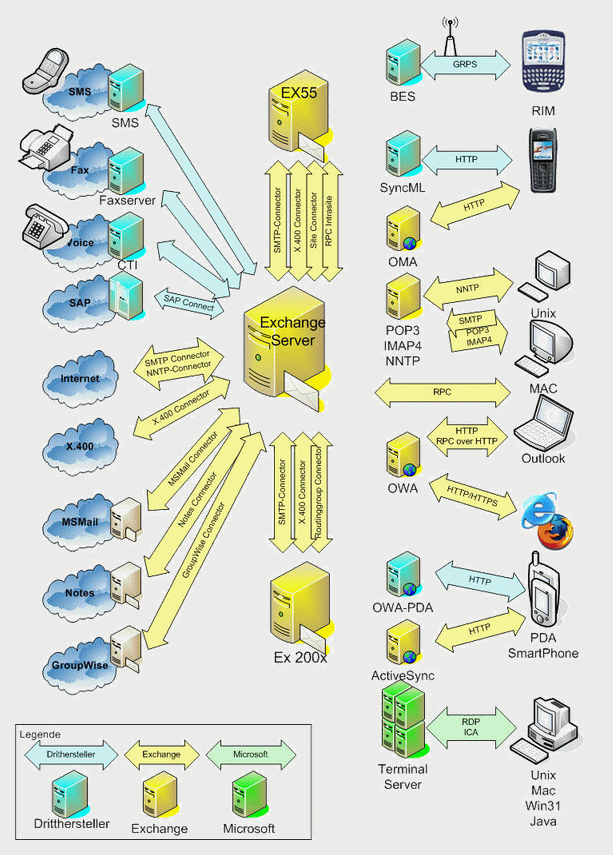
\includegraphics[width=0.70\textwidth]{Abbildungen/Exchange_Verbindungen.png}
\caption*{\\Exchange Verbindungen, Quelle: http://www.msxfaq.de/basics/excomm.htm}
\label{Exchange_Verbindungen}
\end{figure}


\newpage

\begin{flushright}
Anhang 2\\
Blatt 1\\
\end{flushright}

\begin{figure}[h!]
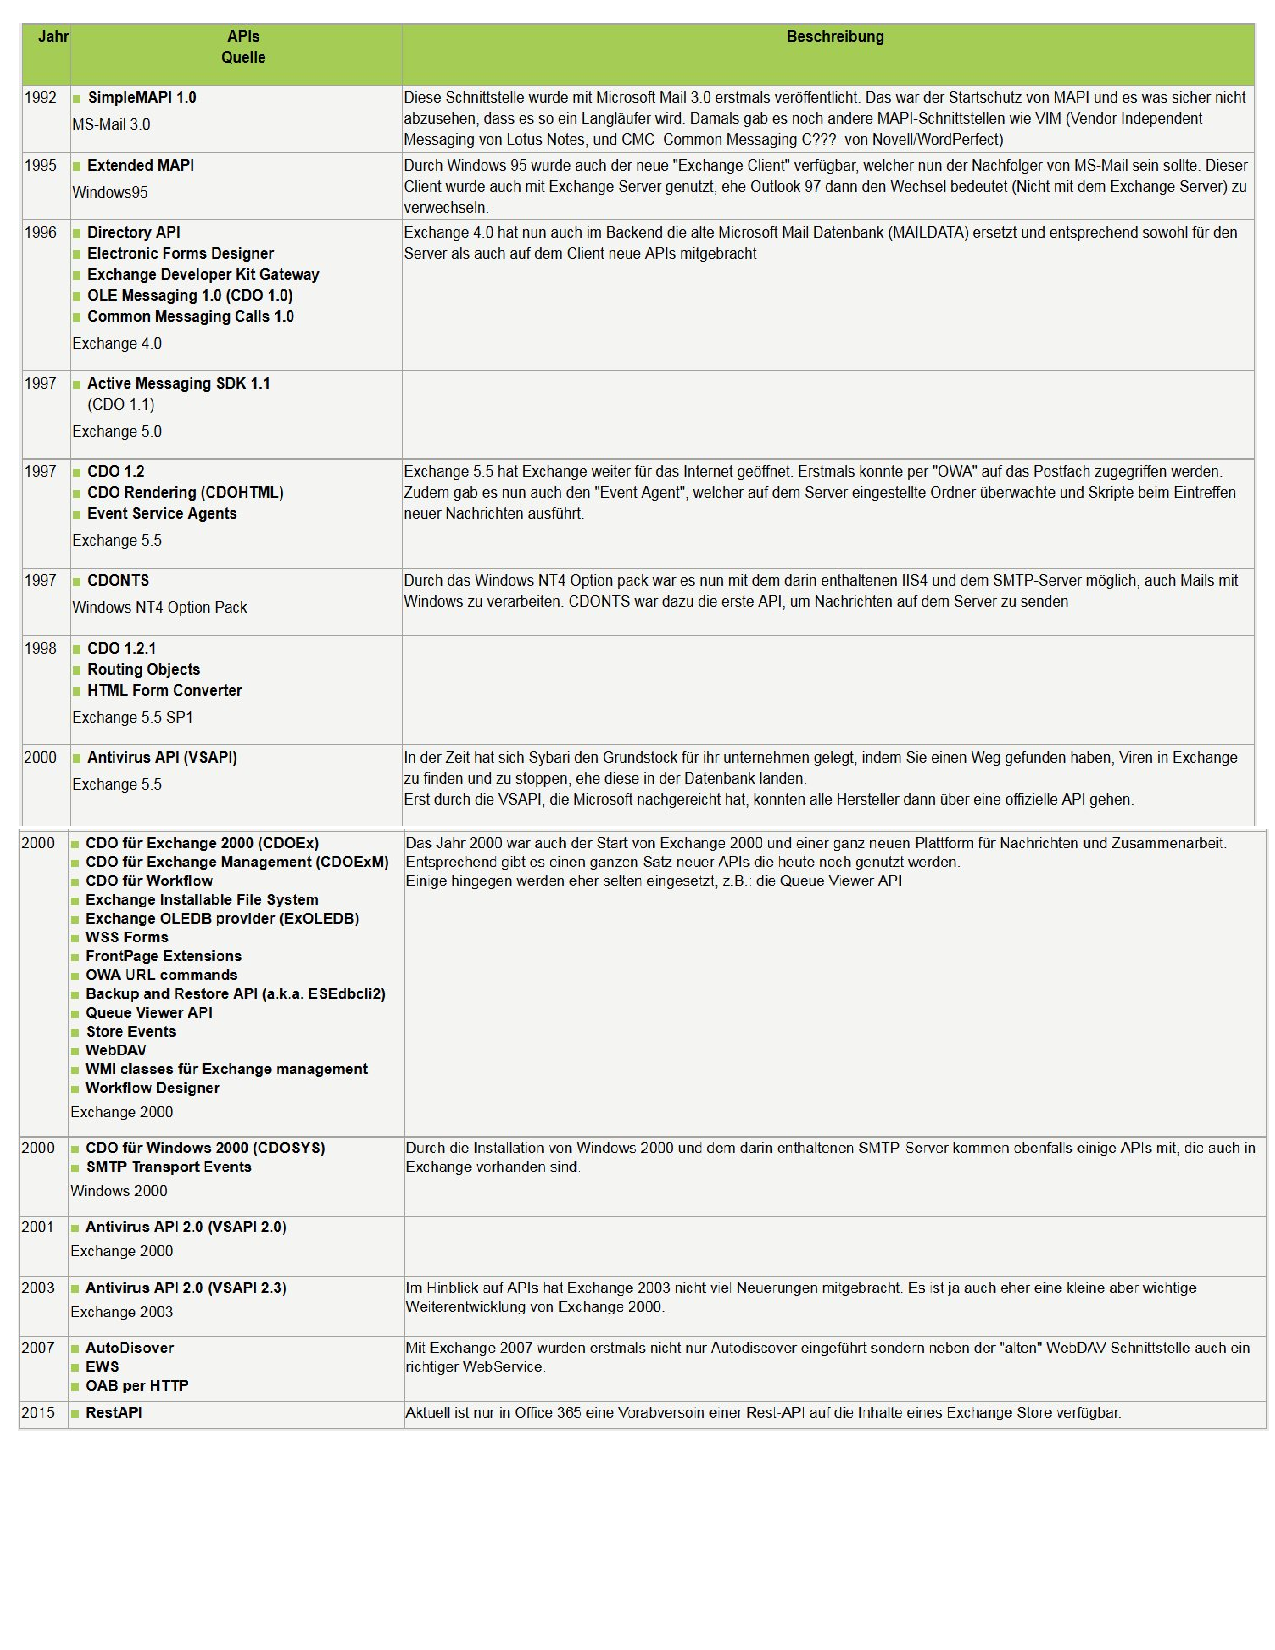
\includegraphics[width=1.0\textwidth]{Abbildungen/API_Geschichte2.pdf}
\caption*{Geschichte der APIs, Quelle: http://www.msxfaq.de/code/wege.htm}
\label{API_Geschichte}
\end{figure}

\newpage

\begin{flushright}
Anhang 3\\
Blatt 1\\
\label{Anhang3_1}
\end{flushright}

\begin{figure}[h!]
\captionsetup{justification=raggedright,
singlelinecheck=false
}
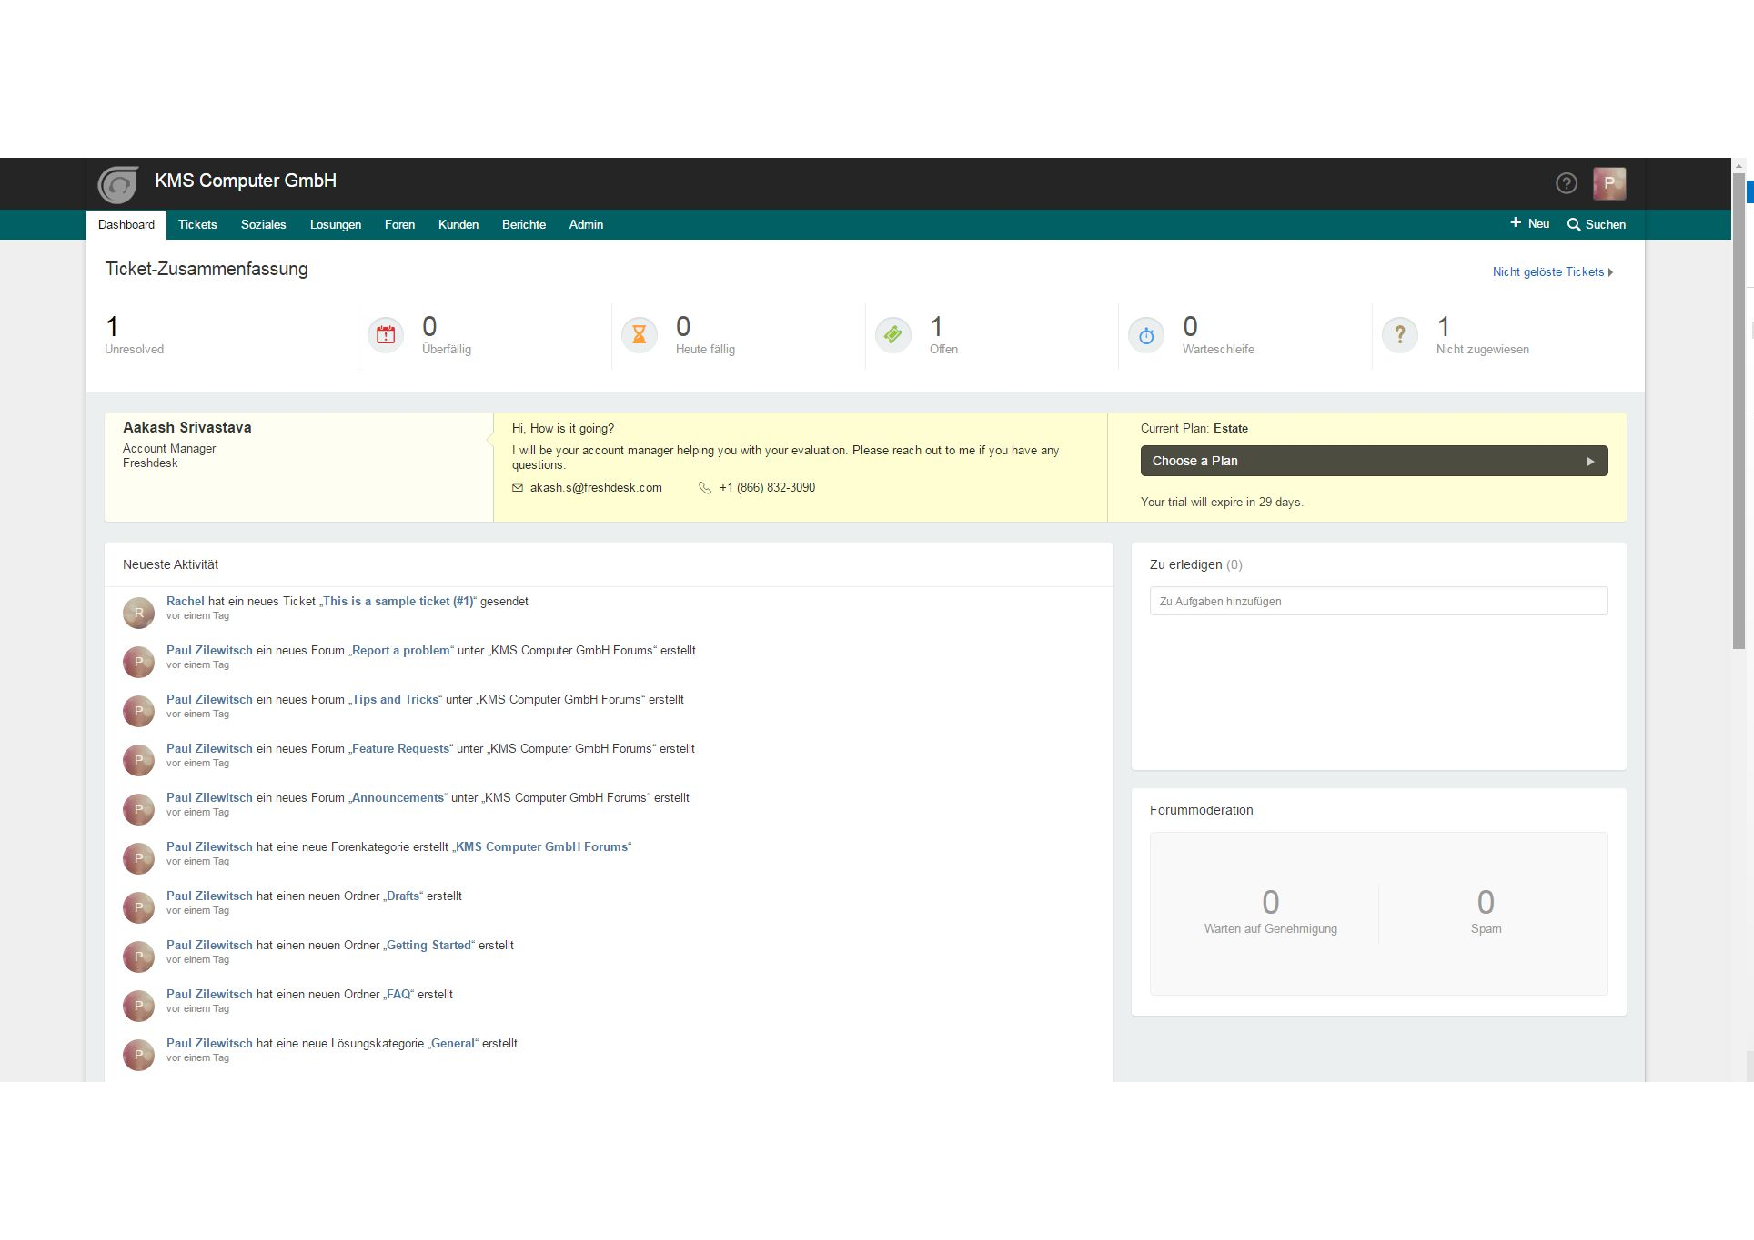
\includegraphics[width=0.85\textwidth]{Abbildungen/Freshdesk.pdf}
\caption*{Screenshot Freshdesk Dashboard, \newline
Quelle: https://kmscomputergmbh.freshdesk.com/helpdesk/dashboard}
\label{Freshdesk}
\end{figure}



\begin{figure}[h!]
\captionsetup{justification=raggedright,
singlelinecheck=false
}
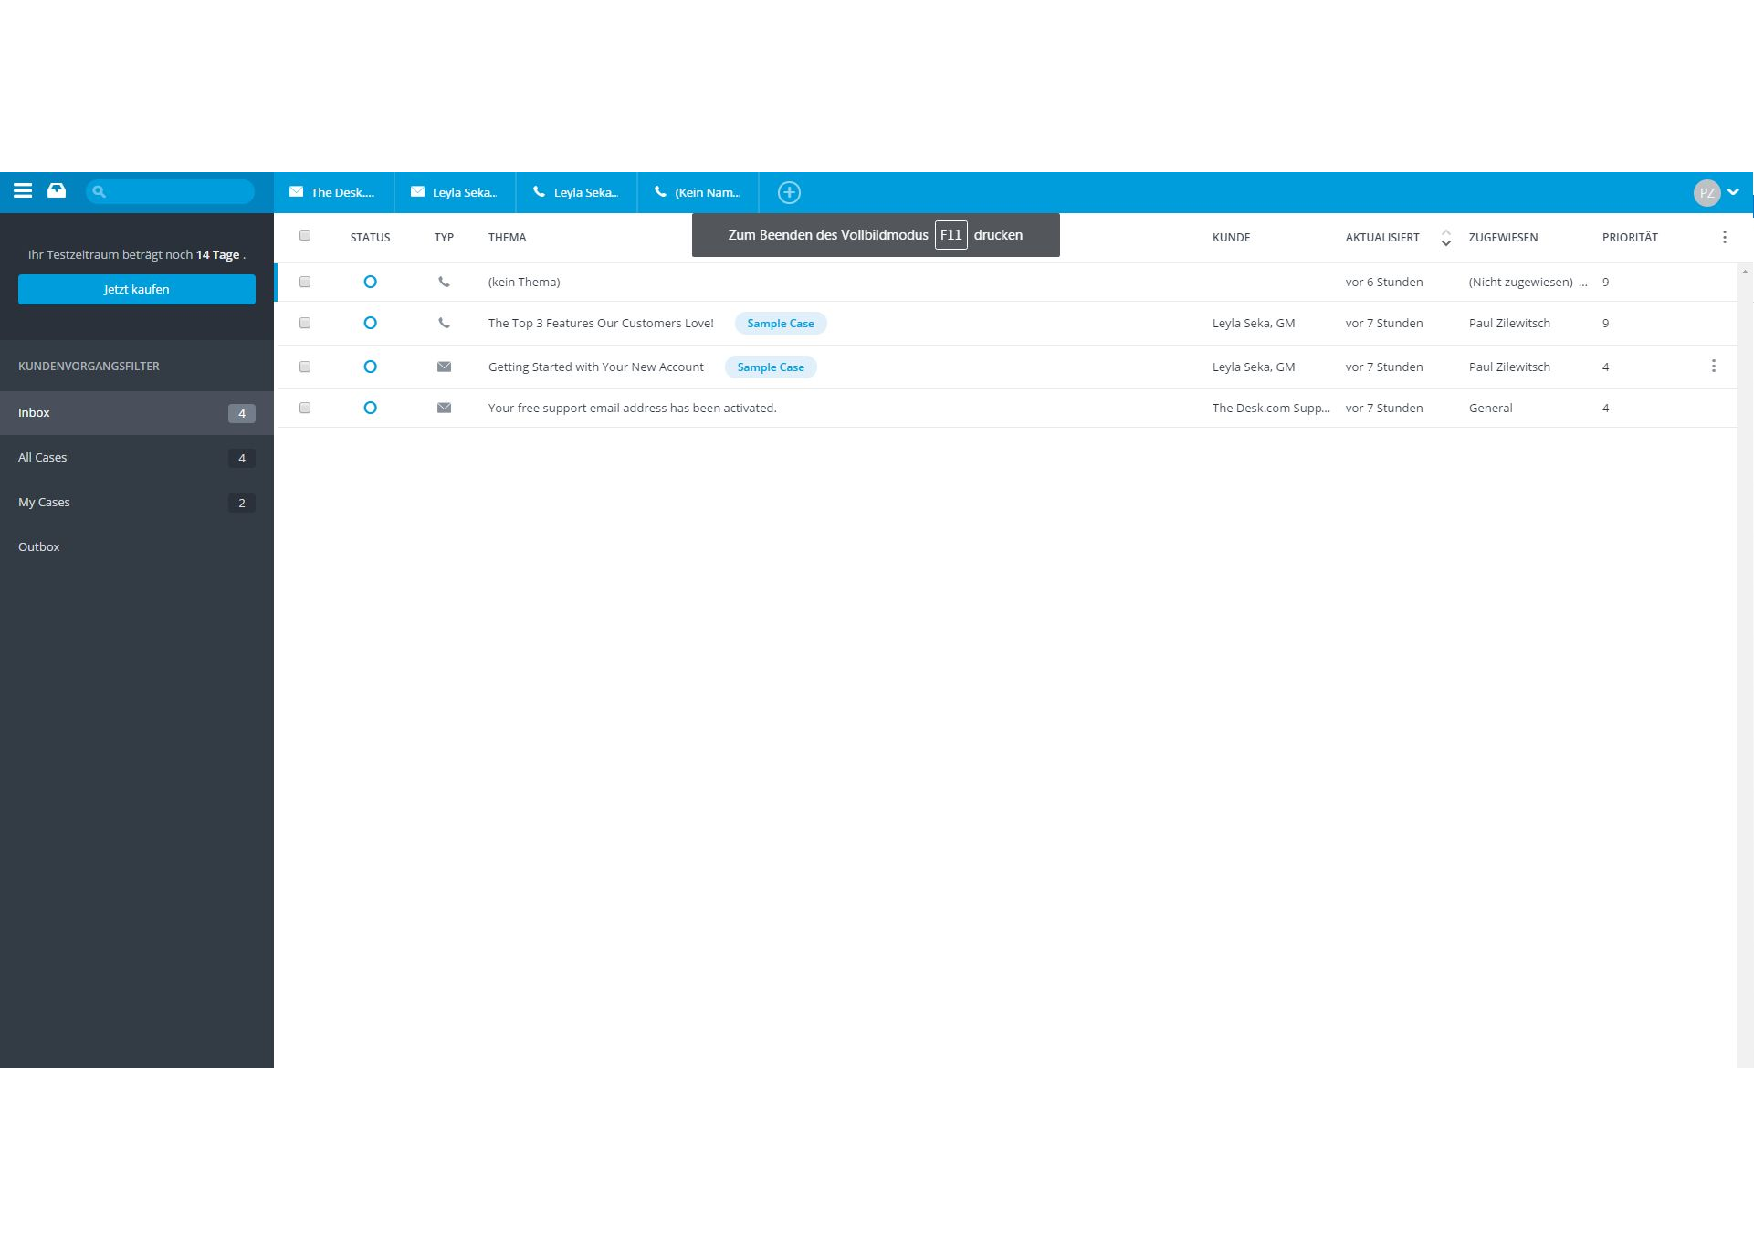
\includegraphics[width=0.85\textwidth]{Abbildungen/Deskcom.pdf}
\caption*{Screenshot Desk.com Dashboard,\newline
Quelle: https://kmscomputergmbh.desk.com/web/agent}
\label{Deskcom}
\end{figure}

\newpage

\begin{flushright}
Anhang 3\\
Blatt 2\\
\label{Anhang3_2}
\end{flushright}


\begin{figure}[h!]
\captionsetup{justification=raggedright,
singlelinecheck=false
}
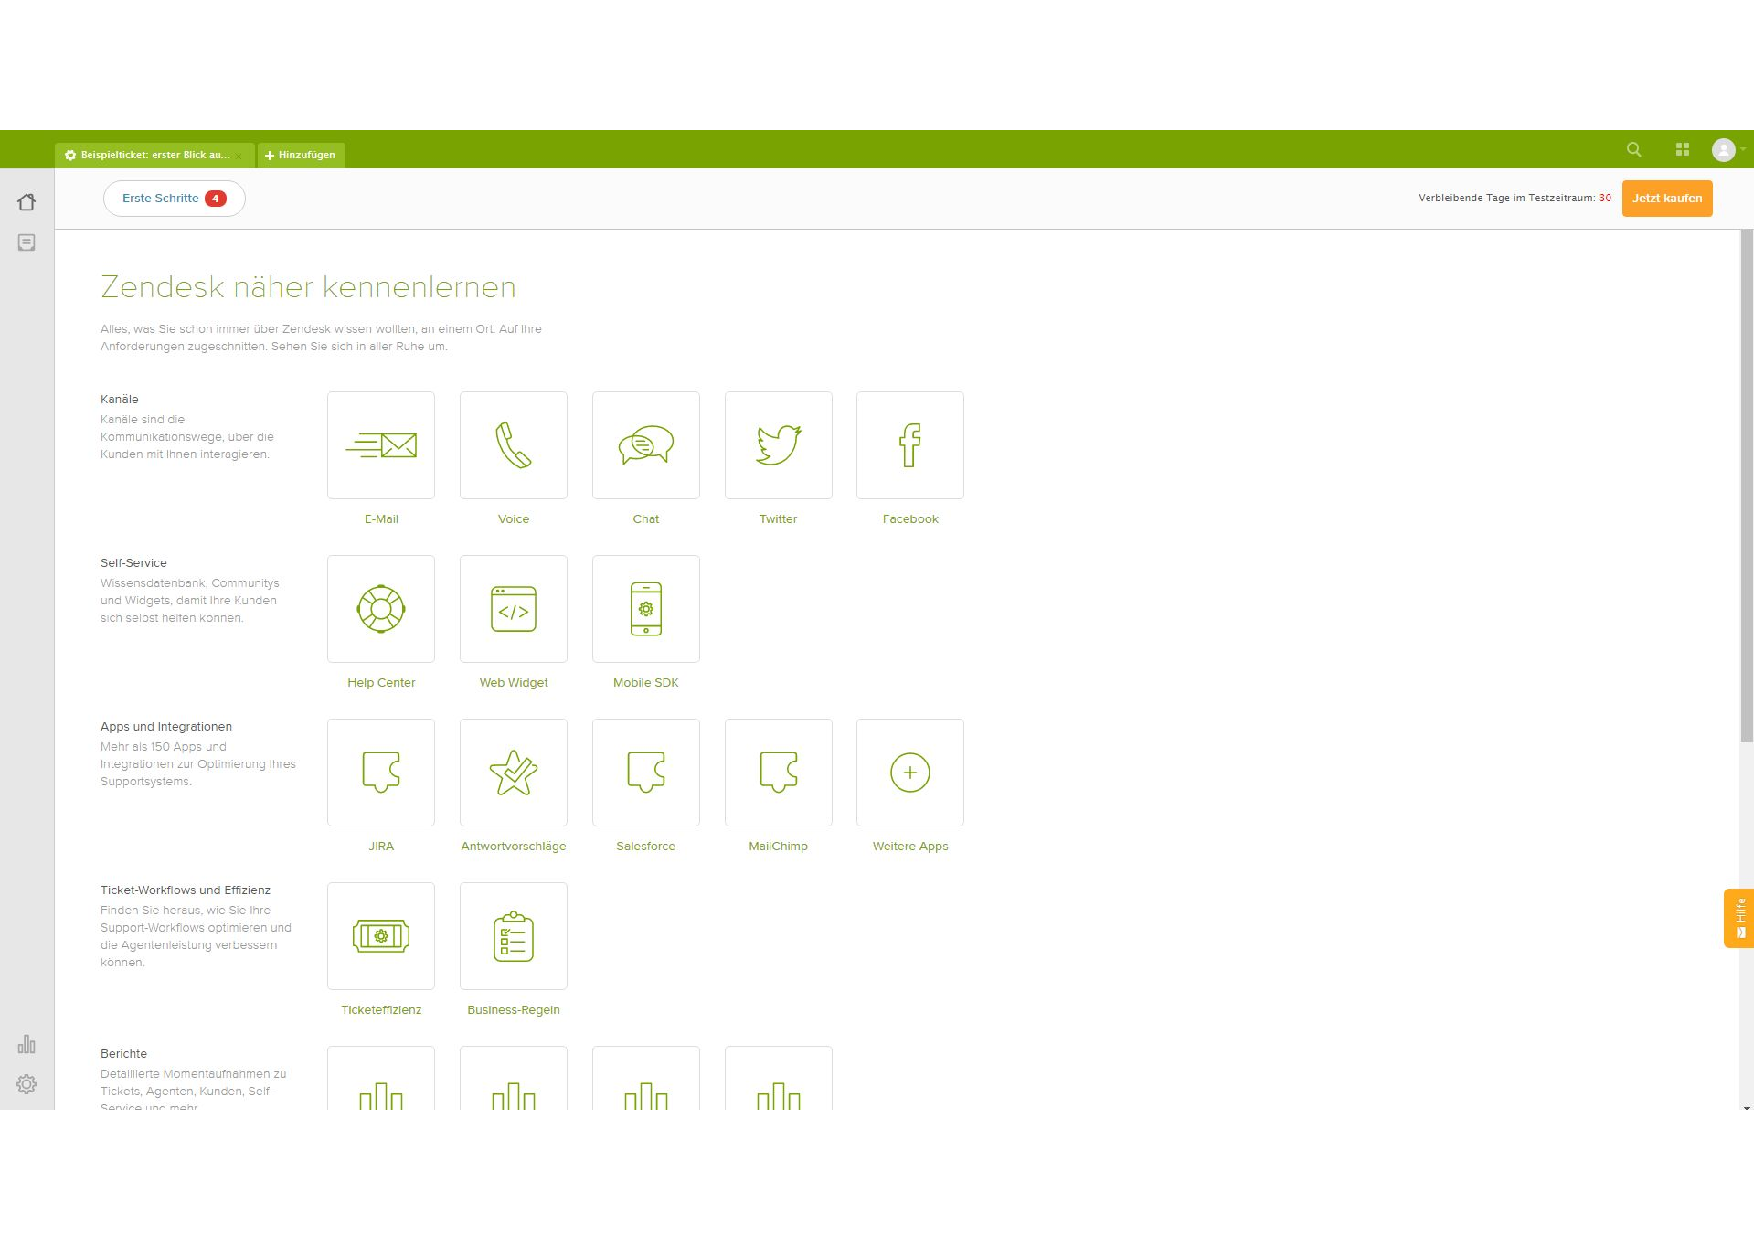
\includegraphics[width=0.85\textwidth]{Abbildungen/Zendesk.pdf}
\caption*{\noindent Screenshot Zendesk Dashboard, \newline
Quelle: https://kmscomputergmbh.zendesk.com/agent/discovery}
\label{Zendesk}
\end{figure}

\begin{figure}[h!]
\captionsetup{justification=raggedright,
singlelinecheck=false
}
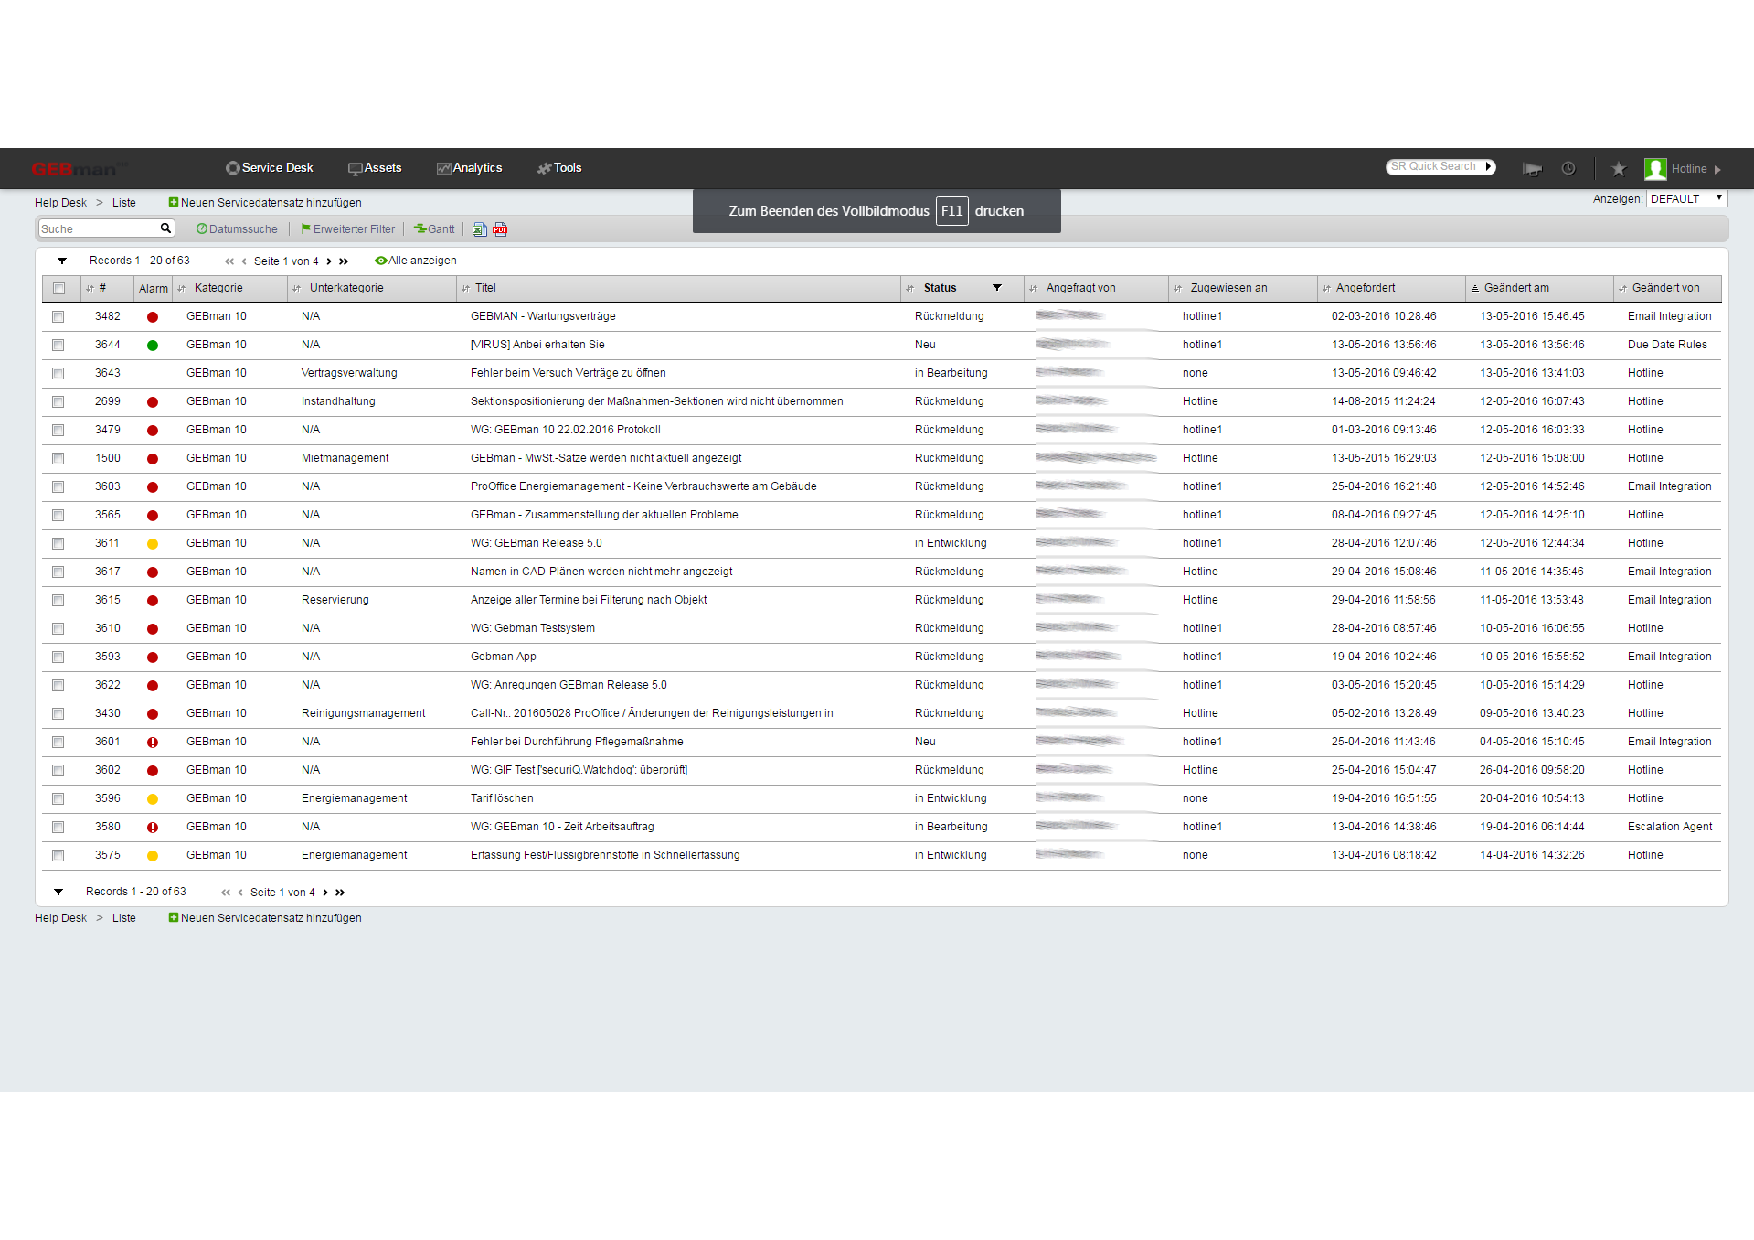
\includegraphics[width=0.85\textwidth]{Abbildungen/SysAid.pdf}
\caption*{Screenshot SysAid Dashboard, \newline
Quelle: \url{http://gebmanhelp.gebman.com:8080/HelpDesk.jsp?helpdeskfrm&fromId=List}}
\label{SysAid}
\end{figure}

\newpage


\begin{flushright}
Anhang 4\\
Blatt 1\\
\label{Anhang4}
\end{flushright}


\begin{figure}[h!]
\captionsetup{justification=raggedright,
singlelinecheck=false
}
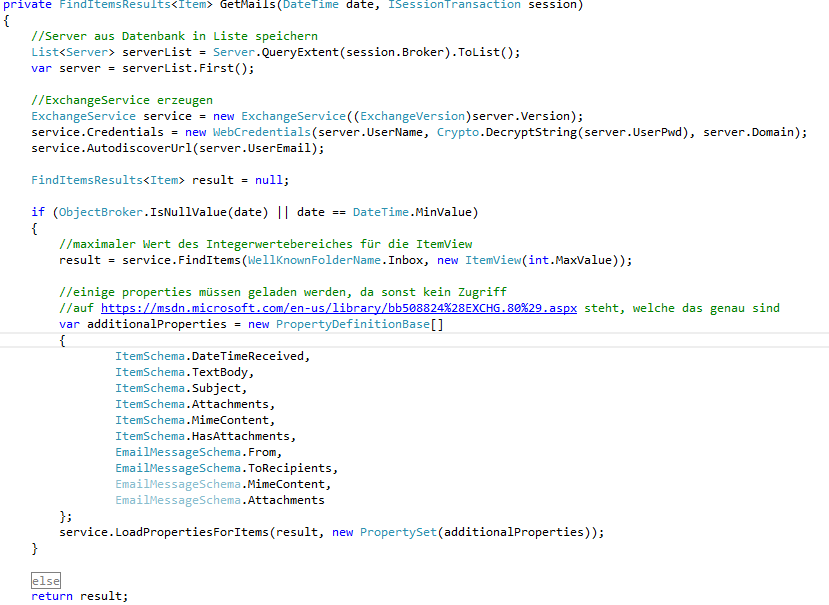
\includegraphics[width=0.95\textwidth]{Abbildungen/Codeausschnitt.png}
	\caption*{\\Codeausschnitt \textit{GetMails( )}, Quelle: eigene Darstellung}
	\label{Codeausschnitt}
\end{figure}








\newpage

%-------------------------------------------------------------------------------------------------------
%					Literaturverzeichnis
%-------------------------------------------------------------------------------------------------------

\addcontentsline{toc}{section}{Literaturverzeichnis}
\bibliography{Literaturverzeichnis/literatur}


%-------------------------------------------------------------------------------------------------------
%					10 Eidestaatliche Erklärung
%-------------------------------------------------------------------------------------------------------

\newpage
 % !TEX root = Bachelorarbeit_Paul_Zilewitsch.tex
\thispagestyle{empty}
\section*{Eidesstattliche Erklärung }
\noindent
Ich erkläre an Eides statt, dass ich die vorliegende Arbeit selbständig und ohne unerlaubte fremde Hilfe angefertigt,  andere  als  die  angegebenen  Quellen  und  Hilfsmittel  nicht  benutzt habe. Die aus fremden Quellen direkt oder indirekt übernommenen Stellen sind als solche kenntlich gemacht. Die Zustimmung des Partnerunternehmens in der Praxis zur Verwendung betrieblicher Unterlagen habe ich eingeholt. Die Arbeit wurde bisher in gleicher oder ähnlicher Form keiner anderen  Prüfungsbehörde  vorgelegt  und  auch  nicht  veröffentlicht.
~\\
~\\
~\\
~\\


\noindent
Ort, Abgabetermin\hfill Unterschrift des Verfassers\\

\noindent
Dresden,  18.07.2016\hfill \_\_\_\_\_\_\_\_\_\_\_\_\_\_\_\_\_\_\_\_\_

\end{document}
